\documentclass[aspectratio=169, 14pt]{beamer}
\input{preamble}

\title{Large Language Models}
\subtitle{A Physicist's Perspective}
\date{MCQST Colloquium, M\"unchen, 27 August 2026}

% --- Placeholder caption for the unit-distance hook (patch later) ---
\newcommand{\unitdistancecaption}{%
  arXiv:2605.20695 \quad\textperiodcentered\quad
  Alon, Bloom, Gowers, Litt, Sawin, Shankar, Tsimerman, Wang, Matchett Wood
  \quad\textperiodcentered\quad May 2026\\[2pt]
  human verification of an OpenAI-generated counterexample}

% --- Reusable grey honesty caption for the synthetic grade figures ---
\newcommand{\synthcaption}{%
  {\small\color{tjo@black!55}%
   Synthetic data, illustrative: reproduces the structure of the
   real six-year analysis.}}

% --- NEW (SPEC-EXTENSION): Dirac notation for the no-cloning ledger ---
\newcommand{\ket}[1]{\lvert #1 \rangle}

% --- NEW (TIMELINE): Whitney has no precomposed U+0151, and no
%     combining hungarumlaut; compose it from the spacing accent. ---
\newcommand{\Erdos}{Erd{\accent"02DD o}s}

% --- NEW (SPEC-EXTENSION C2): patchable attribution for the guide ---
% Replace with the arXiv number once the preprint is posted.
\newcommand{\slopcaption}{%
  {\fontsize{12}{15}\selectfont\mdseries\itshape\color{tjo@black!55}%
   Raise High Your Slop Cannon --- guide in preparation, 2026}}

% =====================================================================
% NEW (TIMELINE): shared machinery for the four figure slides G1--G4.
% Geometry comes from design/timeline-slides-design.md, which specifies
% everything in a 1280x720 design frame.  On a 16cm x 9cm beamer page
%   1 design px = 0.0125 cm,  and  a length of n px = (n/8) mm.
% Font sizes: beamer pt = design px * 0.3543.
% =====================================================================

% --- Extra colour roles (design doc SS1.3); palette itself unchanged ---
\definecolor{tjo@red}{HTML}{AA3333}
\definecolor{tjo@muted}{HTML}{5B6B74}
\definecolor{tjo@faint}{HTML}{8A969C}
\definecolor{tjo@rule}{HTML}{C7CFD3}
\definecolor{tjo@ink}{HTML}{1A1E21}
\definecolor{tjo@swe}{HTML}{4A575E}
\definecolor{tjo@future}{HTML}{B6C0C5}
\definecolor{tjo@physbg}{HTML}{F2FAFE}

% --- Letter-spacing helper (fontspec/LuaTeX): \lsp{13}{TEXT} ---
\newcommand{\lsp}[2]{{\addfontfeature{LetterSpace=#1}#2}}

% --- Design-frame picture: origin = page north west, y grows downward,
%     coordinates written directly in design px. ---
\newenvironment{designframe}[1][]
  {\begin{tikzpicture}[remember picture, overlay,
      shift={(current page.north west)}, x=0.0125cm, y=-0.0125cm, #1]}
  {\end{tikzpicture}}

% --- Shared chrome for the four figure slides: title + cyan rule ---
\newcommand{\dftitle}[1]{%
  \node[anchor=north west, text=tjo@darkteal,
        font=\fontsize{11.3}{13.5}\selectfont\bfseries] at (40,34) {#1};
  \fill[tjo@cyan, rounded corners=0.25mm] (40,94) rectangle (106,98);}

\begin{document}

% =====================================================================
% TITLE
% =====================================================================

\begin{frame}[plain]
  \titlepage
\end{frame}

% =====================================================================
% PART 1: WHY THIS TALK?
% =====================================================================

\sectiondivider{Why this talk?}

% --- Hook A: unit-distance problem (asset produced in parallel) ---
\begin{frame}[plain]
  \vfill
  \centering
  \IfFileExists{assets/unitdistance_pr.png}{%
    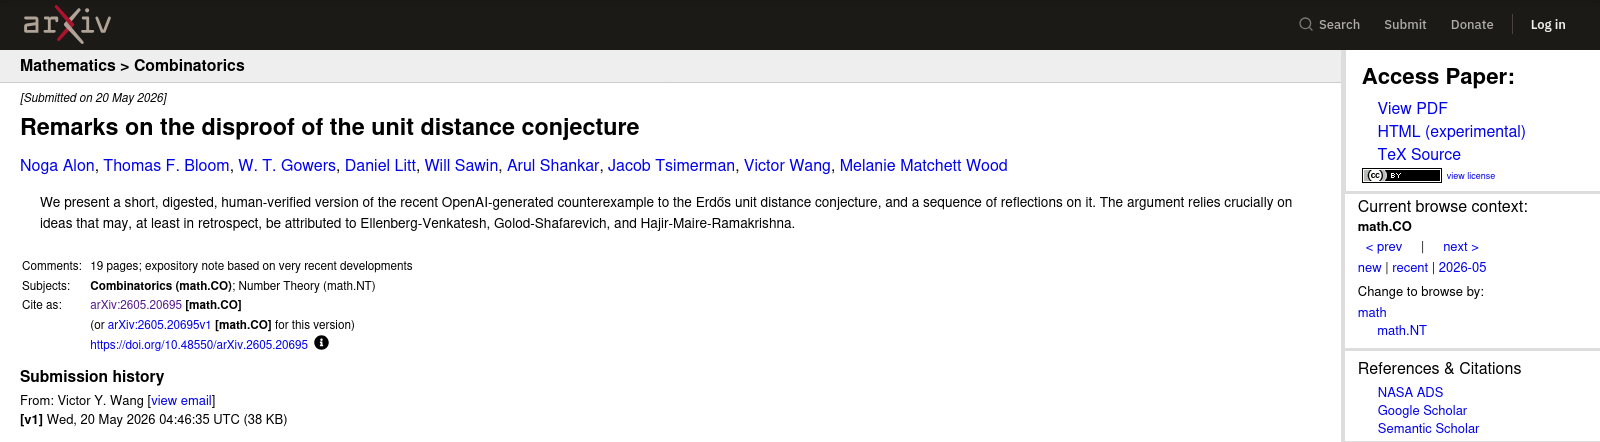
\includegraphics[width=0.82\textwidth]{assets/unitdistance_pr.png}%
  }{%
    % SPEC-DEVIATION: asset is being produced in parallel; show a
    % visible placeholder so the deck always compiles.
    \begin{tikzpicture}
      \draw[tjo@darkteal, line width=1.5pt, rounded corners=6pt]
        (0,0) rectangle (10,5.6);
      \node[align=center, text=tjo@black!55, font=\large] at (5,2.8)
        {\textbf{[ assets/unitdistance\_pr.png ]}\\[0.6em]
         full-bleed press screenshot\\ (produced in parallel)};
    \end{tikzpicture}%
  }

  \vskip1em
  {\small\color{tjo@black!60}\unitdistancecaption}
  \vfill
\end{frame}

% --- Hook B: the GPT-5.2 amplitudes paper ---
% ERRATUM (TIMELINE design doc SS0): this is NOT a string-theory paper.
% "Single-minus gluon tree amplitudes are nonzero" is a tree-level
% gauge-theory amplitudes result (Guevara, Lupsasca, Skinner,
% Strominger, Weil).  There is no IAS author.
\begin{frame}[plain]
  \vfill
  \centering
  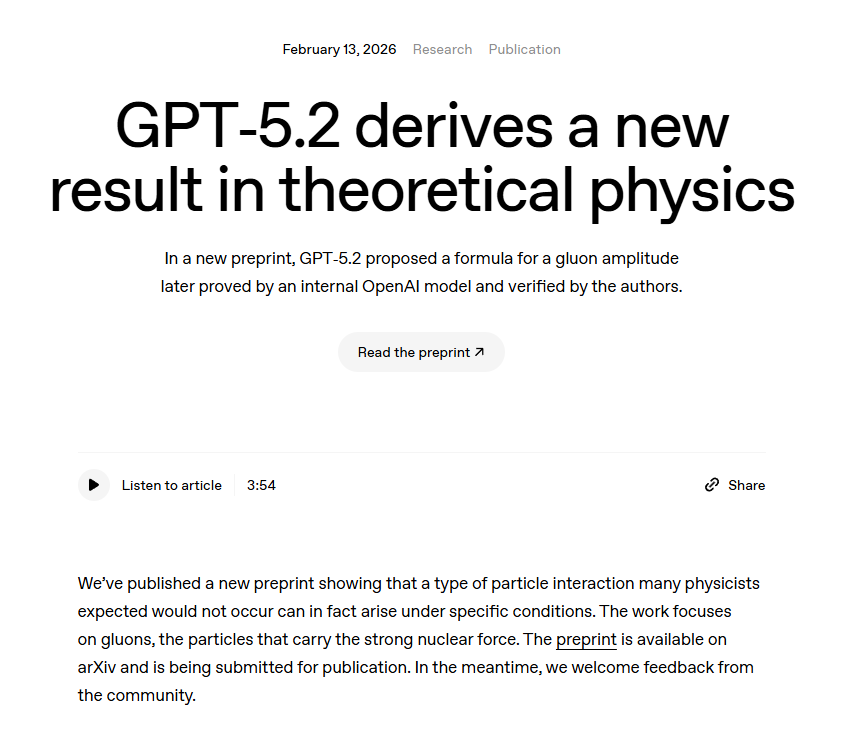
\includegraphics[width=0.58\textwidth]{assets/gpt52pr.PNG}

  \vskip0.8em
  {\small\color{tjo@black!60}%
    arXiv:2602.12176 \enspace\textperiodcentered\enspace
    Harvard, Vanderbilt, Cambridge, OpenAI \enspace\textperiodcentered\enspace
    February 2026\\[2pt]
    gauge-theory scattering amplitudes ---\\[1pt]
    GPT-5.2 conjectured the closed form and proved it}
  \vfill
\end{frame}

% NEW (TIMELINE G3)
% Verification-tier ledger.  Geometry: design doc SS4.
\begin{frame}[plain]
\begin{designframe}[%
  badge/.style={anchor=north west, inner sep=0pt, minimum width=7.25mm,
    minimum height=2.75mm, rounded corners=0.75mm, text=white,
    font=\fontsize{4.6}{5.5}\selectfont\bfseries, align=center},
  leg/.style={anchor=west, text=tjo@muted,
    font=\fontsize{5.1}{6.4}\selectfont},
  rdate/.style={anchor=west, text=tjo@darkteal,
    font=\fontsize{5.1}{6.4}\selectfont\bfseries},
  rtext/.style={anchor=west, text=tjo@ink,
    font=\fontsize{5.6}{7}\selectfont},
]
  \dftitle{The flurry --- and how much of it is checked}

  % ---------- tier legend ----------
  \node[badge, fill=tjo@green]   at (40,110)  {T1};
  \node[leg] at (106,121) {machine-checked or officially graded};
  \node[badge, fill=tjo@medblue] at (393,110) {T2};
  \node[leg] at (458,121) {arXiv --- named humans read it};
  \node[badge, fill=tjo@red]     at (703,110) {T3};
  \node[leg] at (770,121) {announced only, no referee};

  % ---------- tinted band behind the two physics rows ----------
  \fill[tjo@physbg, rounded corners=0.875mm] (34,236) rectangle (836,322);
  \fill[tjo@cyan] (34,239) rectangle (37,319);
  \node[anchor=east, text=tjo@cyan,
        font=\fontsize{4.3}{5.4}\selectfont\bfseries] at (836,257)
    {\lsp{16}{PHYSICS}};

  % ---------- the eight results ----------
  \node[badge, fill=tjo@green]   at (40,160.5) {T1};
  \node[rdate] at (110,171.5) {Jul 2025};
  \node[rtext] at (203,171.5)
    {IMO gold, in natural language, officially graded};

  \node[badge, fill=tjo@green]   at (40,203.5) {T1};
  \node[rdate] at (110,214.5) {Jan 2026};
  \node[rtext] at (203,214.5)
    {\Erdos\ \#728 --- first autonomous solve, with a Lean certificate};

  \node[badge, fill=tjo@medblue] at (40,246.5) {T2};
  \node[rdate] at (110,257.5) {Feb 2026};
  \node[rtext] at (203,257.5)
    {Gauge-theory amplitudes --- GPT-5.2 and five named physicists};

  \node[badge, fill=tjo@medblue] at (40,289.5) {T2};
  \node[rdate] at (110,300.5) {Mar 2026};
  \node[rtext] at (203,300.5)
    {Bethe ansatz, two new integrable chains --- checked vs exact
     diagonalisation};

  \node[badge, fill=tjo@medblue] at (40,332.5) {T2};
  \node[rdate] at (110,343.5) {May 2026};
  \node[rtext] at (203,343.5)
    {Unit distance disproved --- nine mathematicians read it line by line};

  \node[badge, fill=tjo@green]   at (40,375.5) {T1};
  \node[rdate] at (110,386.5) {May 2026};
  \node[rtext] at (203,386.5)
    {AlphaProof Nexus: 9 \Erdos{} $+$ 44 OEIS, Lean, a few hundred \$ each};

  \node[badge, fill=tjo@red]     at (40,418.5) {T3};
  \node[rdate] at (110,429.5) {Jul 2026};
  \node[rtext] at (203,429.5)
    {Jacobian conjecture false in dim $\geq 3$ --- announced in one post on X};

  \node[badge, fill=tjo@green]   at (40,461.5) {T1*};
  \node[rdate] at (110,472.5) {Aug 2026};
  \node[rtext] at (203,472.5)
    {``Astra'': ten decade-open problems, Lean, ${<}\,\$2$k each ---
     {\bfseries\color{tjo@red} zero referees}};

  % ---------- the Jacobian announcement, verbatim ----------
  \fill[tjo@codebg, rounded corners=1mm] (34,504) rectangle (836,580);
  \fill[tjo@cyan] (34,506) rectangle (39,578);
  \node[anchor=north west, text=tjo@darkteal,
        font=\fontsize{8}{10}\selectfont\ttfamily\bfseries] at (52,514)
    {\textquotedblleft hello there the jacobian conjecture is false
     thanx\textquotedblright};
  \node[anchor=north west, text=tjo@muted,
        font=\fontsize{4.7}{5.9}\selectfont] at (52,545)
    {the entire public announcement, 20 Jul 2026 --- an 87-year-old
     conjecture, checked by hand within days};

  % ---------- the denominator ----------
  \draw[tjo@lightgrey, line width=0.125mm] (848,150) -- (848,578);

  \node[anchor=north west, text=tjo@darkteal,
        font=\fontsize{6.7}{8.4}\selectfont\bfseries] at (862,150)
    {\ldots{}and the denominator};
  \node[anchor=north west, text=tjo@muted, text width=47.25mm,
        font=\fontsize{5}{6.6}\selectfont] at (862,180)
    {The community's own tracker marks every AI contribution:};

  \fill[tjo@green] (869,238) circle[radius=0.9375mm];
  \node[anchor=west, text=tjo@ink, font=\fontsize{5.1}{6.4}\selectfont]
    at (886,238) {full resolution};

  \begin{scope}
    \clip (860,260) rectangle (869,276);
    \fill[tjo@green] (869,268) circle[radius=0.9375mm];
  \end{scope}
  \draw[tjo@green, line width=0.2mm] (869,268) circle[radius=0.9375mm];
  \node[anchor=west, text=tjo@ink, font=\fontsize{5.1}{6.4}\selectfont]
    at (886,268) {partial progress};

  \fill[tjo@red] (869,298) circle[radius=0.9375mm];
  \node[anchor=west, text=tjo@ink,
        font=\fontsize{5.1}{6.4}\selectfont\bfseries]
    at (886,298) {incorrect work};

  \draw[tjo@black!35, line width=0.25mm, fill=white]
    (869,328) circle[radius=0.9375mm];
  \node[anchor=west, text=tjo@ink,
        font=\fontsize{5.1}{6.4}\selectfont\bfseries]
    at (886,328) {unverified --- never read};

  \draw[tjo@lightgrey, line width=0.125mm] (862,355) -- (1240,355);

  \node[anchor=north west, text=tjo@darkteal, text width=47.25mm,
        font=\fontsize{5.3}{7}\selectfont\itshape] at (862,368)
    {``AI is being used a lot by people who aren't
      mathematicians\ldots{} no human has read it.''};
  \node[anchor=north west, text=tjo@muted,
        font=\fontsize{4.6}{5.8}\selectfont] at (862,418)
    {--- Thomas Bloom, curator, erdosproblems.com};

  \node[anchor=north west, text=tjo@cyan,
        font=\fontsize{10.6}{13}\selectfont\bfseries] at (862,478)
    {1 in 277};
  \node[anchor=north west, text=tjo@muted, text width=47.25mm,
        font=\fontsize{4.8}{6.3}\selectfont] at (862,522)
    {arXiv submissions flagged as unvetted LLM output, early 2026.
     Now a one-year ban.};

  % ---------- summary ----------
  \node[anchor=north, align=center, text=tjo@darkteal,
        font=\fontsize{8.5}{11}\selectfont\bfseries] at (640,598)
    {Generation has been automated faster than verification ---\\
     and the gap is the whole story.};
\end{designframe}
\end{frame}

% --- Hook C1: grade decorrelation --- a control experiment run on us ---
\begin{frame}{A control experiment, run on us}
  \begin{flushleft}
  \hspace{1.5em}First-year theoretical physics, six years of grades

  \vskip0.5em
  \hspace{1.5em}Weekly take-home assignment, out of 100
  {\color{tjo@black!55} (unsupervised)}

  \vskip0.5em
  \hspace{1.5em}Invigilated final exam, out of 10
  {\color{tjo@black!55} (the control)}

  \vskip0.5em
  \hspace{1.5em}2020--2023: the two agree at $b \approx 0.10$
  \end{flushleft}

  \vskip0.8em
  \centering
  {\color{tjo@darkteal}\bfseries
    When the link breaks, it is the assignment that broke, not the exam}

  \vskip0.6em
  \synthcaption
\end{frame}

% --- Hook C2: 2020 baseline ---
\begin{frame}{2020: the instruments agree}
  \centering
  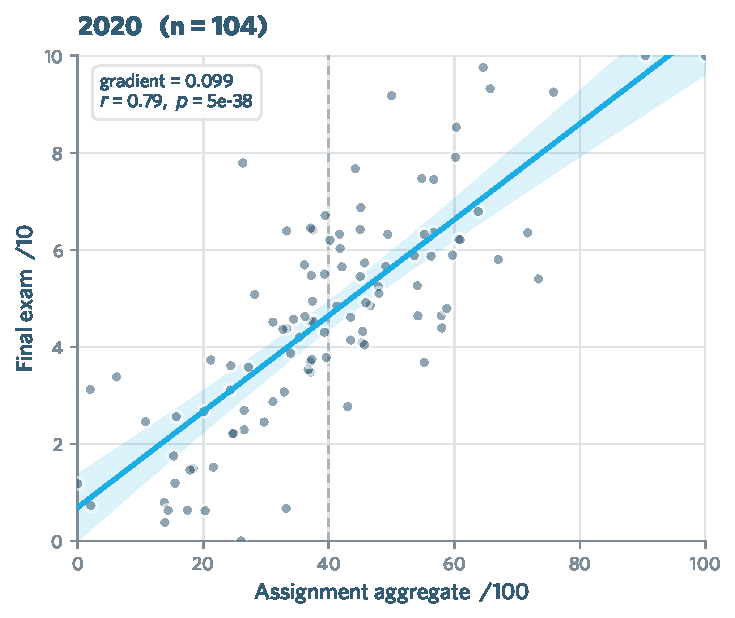
\includegraphics[height=0.52\textheight]{../grade-decorrelation/figures/scatter_2020.pdf}

  \vskip0.4em
  {\small\color{tjo@darkteal}\bfseries
    $b = 0.099$, $r = 0.79$:} {\small the assignment predicts the exam}

  \vskip0.3em
  \synthcaption
\end{frame}

% --- Hook C3: 2025 collapse ---
\begin{frame}{2025: the link is gone}
  \centering
  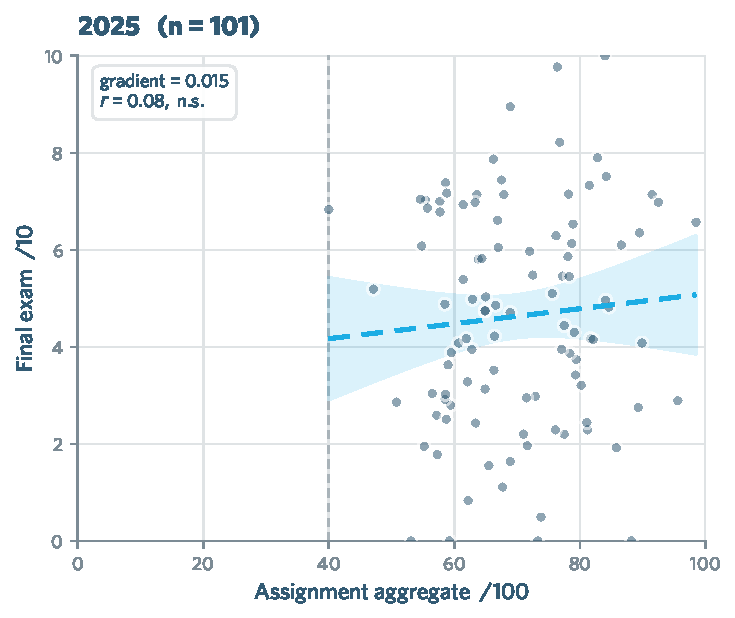
\includegraphics[height=0.52\textheight]{../grade-decorrelation/figures/scatter_2025.pdf}

  \vskip0.4em
  {\small\color{tjo@darkteal}\bfseries
    $b = 0.015$, $r = 0.08$, n.s.:} {\small it no longer measures what the
  exam measures}

  \vskip0.3em
  \synthcaption
\end{frame}

% --- Hook C4: the collapse in one image (punchline) ---
\begin{frame}{The collapse, one panel per year}
  \centering
  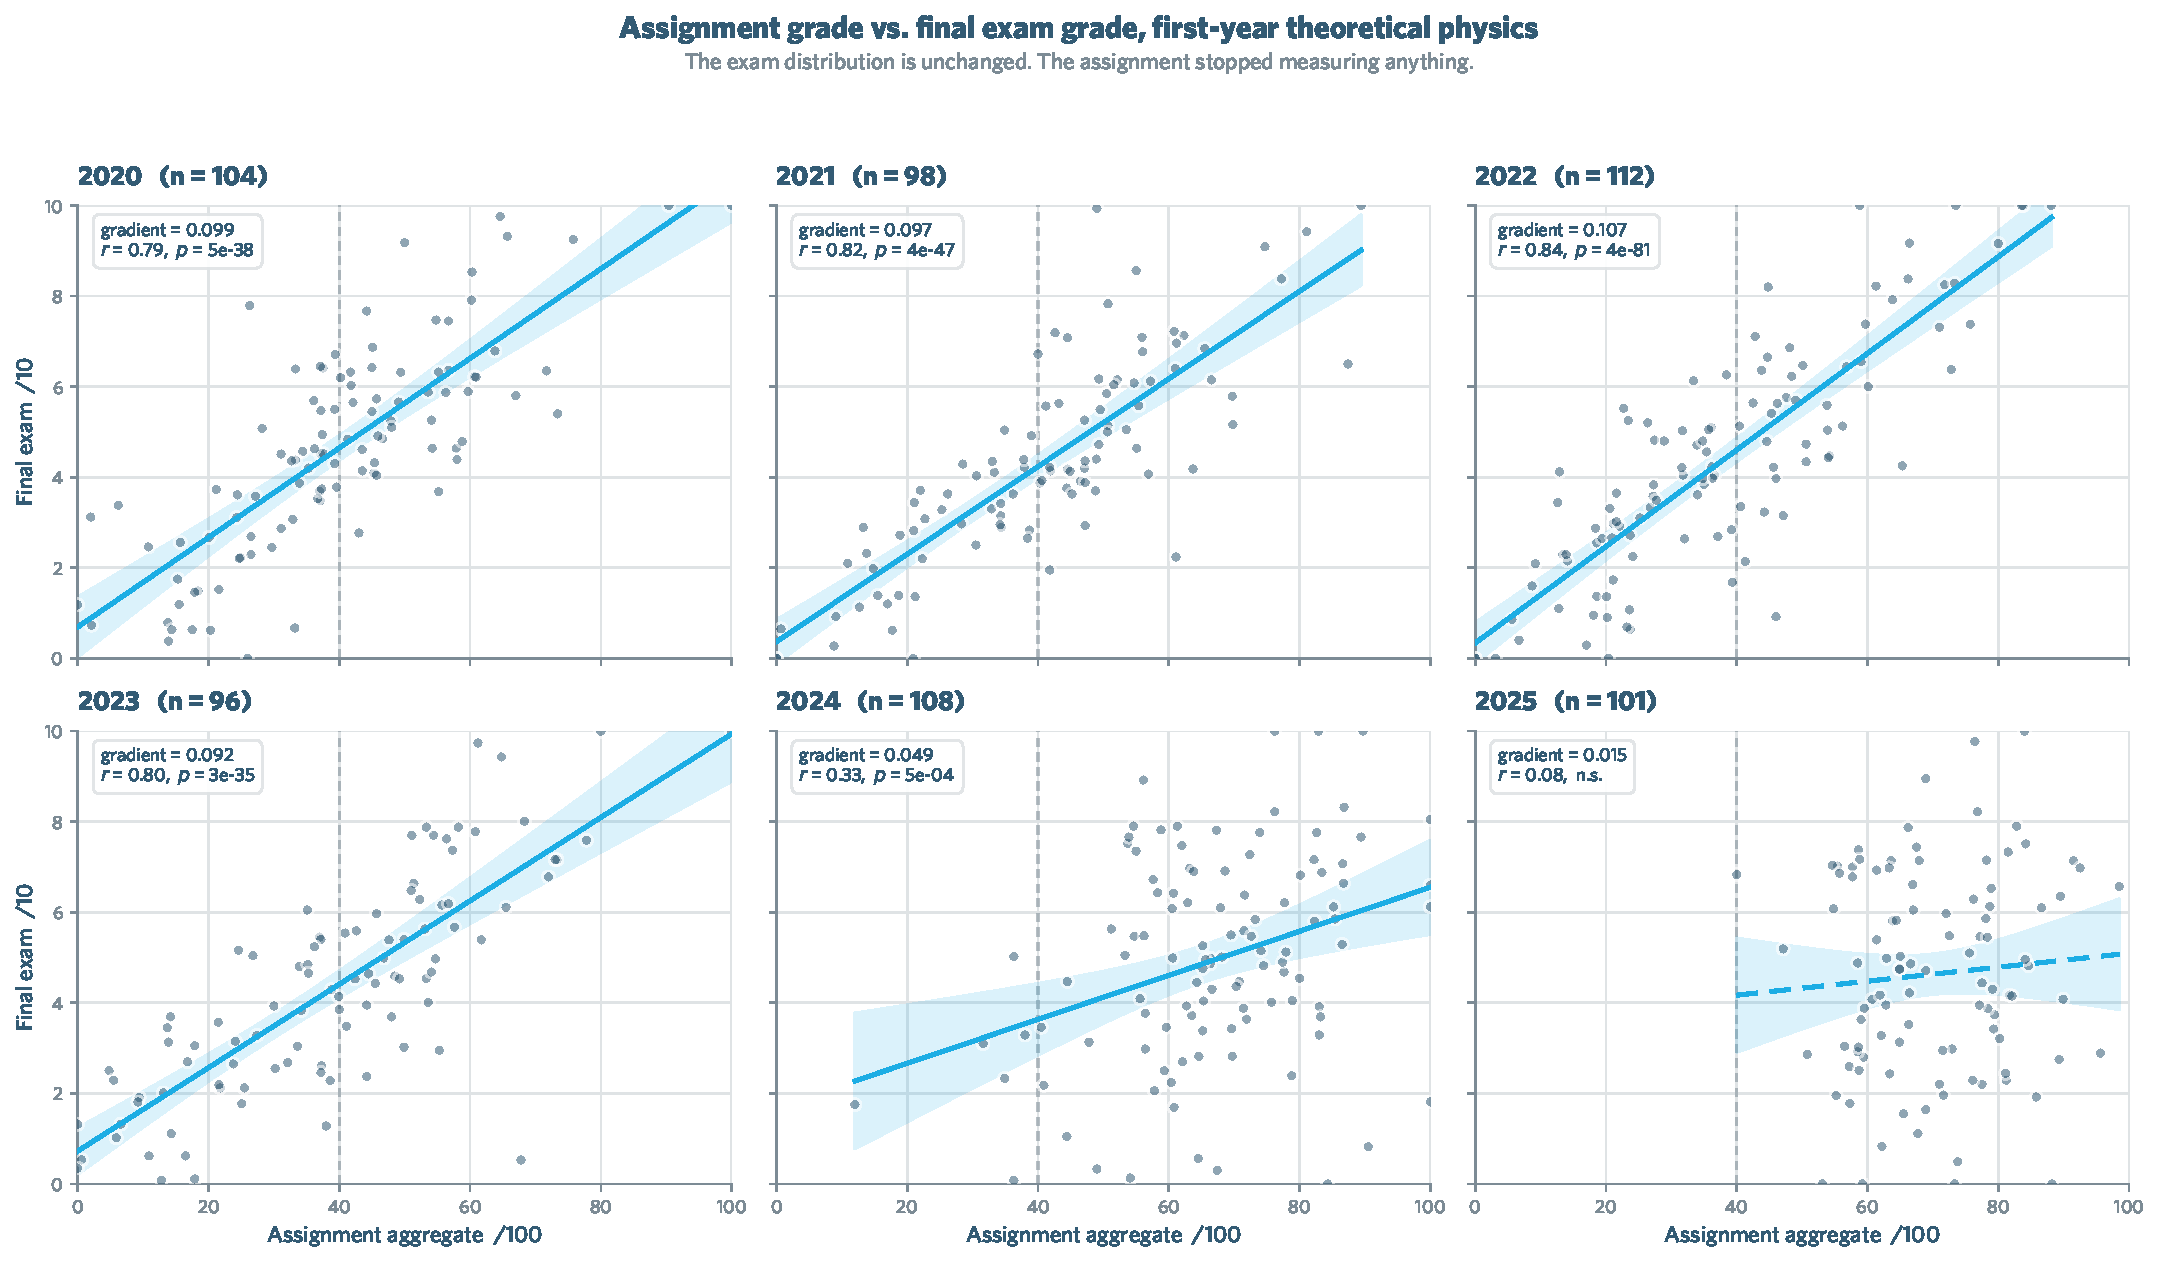
\includegraphics[height=0.40\textheight]{../grade-decorrelation/figures/scatter_grid.pdf}

  \vskip0.2em
  {\footnotesize\color{tjo@darkteal}\bfseries
    Pooled interaction $d = -0.063$, $p \approx 1\times10^{-7}$:} {\footnotesize
  adoption is uncorrelated with ability}

  \vskip0.15em
  \synthcaption
\end{frame}

% --- Audience survey (adapted from seminar deck) ---
\begin{frame}{Quick survey: hands up}
  \vfill
  \centering
  {\fontsize{20}{30}\selectfont
    \begin{tabular}{l}
      \color{tjo@cyan}$\bullet$\quad Who has used ChatGPT, Claude, or Gemini? \\[0.9em]
      \color{tjo@cyan}$\bullet$\quad Who has used one for research? \\[0.9em]
      \color{tjo@cyan}$\bullet$\quad Who has used a coding agent? \\
    \end{tabular}
  }
  \vfill
\end{frame}

% --- Timeline: four moments (extends GC deck's three-moment timeline) ---
\begin{frame}{Four moments}
  \vfill
  \centering
  \begin{tikzpicture}[
    event/.style={
      tjo box,
      minimum width=2.7cm,
      minimum height=1.7cm,
      font=\footnotesize,
      align=center,
    },
  ]
    \draw[tjo@black!20, line width=2pt] (-6.7,0) -- (6.7,0);

    \node[event, fill=tjo@lightgrey] at (-5.2,0) {%
      {\bfseries\small\color{tjo@darkteal} Nov 2022}\\[3pt]
      ChatGPT\\launches
    };
    \node[event, fill=tjo@lightgrey] at (-1.7,0) {%
      {\bfseries\small\color{tjo@darkteal} Q1 2025}\\[3pt]
      Claude Code,\\Cursor, Copilot
    };
    \node[event, fill=tjo@lightgrey] at (1.7,0) {%
      {\bfseries\small\color{tjo@darkteal} Q4 2025}\\[3pt]
      Opus 4.5, GPT-5.2\\cross a threshold
    };
    \node[event, fill=tjo@cyan!25] at (5.2,0) {%
      {\bfseries\small\color{tjo@darkteal} Q2 2026}\\[3pt]
      Fable 5, GPT-5.6,\\GLM-5.2
    };
  \end{tikzpicture}
  \vfill
\end{frame}

% NEW (TIMELINE G1)
% Five stages of AI grief.  Geometry: design doc SS2.
% Stage colours: shock = cyan, anger = red, bargaining = medblue,
% depression = darkteal, acceptance = green.
\begin{frame}[plain]
\begin{designframe}[%
  dt/.style={anchor=north, font=\fontsize{5.3}{6.6}\selectfont\bfseries},
  ev/.style={anchor=north, align=center, text width=26mm, text=tjo@ink,
             font=\fontsize{5.7}{7.4}\selectfont},
  stem/.style={line width=0.2mm},
]
  \dftitle{The five stages of AI grief}
  \node[anchor=north east, align=right, text=tjo@muted,
        font=\fontsize{5.7}{7.4}\selectfont] at (1240,58)
    {software engineering\\ Nov 2022 $\to$ Jul 2026};

  % ---------- spine, year separators, year labels ----------
  \draw[tjo@lightgrey, line width=0.375mm] (44,366) -- (1236,366);
  \foreach \x in {185,527,983}
    \draw[tjo@rule, line width=0.175mm, dash pattern=on 0.4mm off 0.4mm]
      (\x,344) -- (\x,390);
  \foreach \x/\y in {114/2022--23, 290/2024, 755/2025, 1110/2026}
    \node[anchor=north, text=tjo@faint,
          font=\fontsize{4.6}{5.8}\selectfont] at (\x,373) {\y};

  % ---------- events (odd ranks above the spine) ----------
  \draw[stem, tjo@cyan] (128,334) -- (128,366);
  \node[dt, text=tjo@cyan] at (128,266) {Nov 2022};
  \node[ev] at (128,290) {ChatGPT launches --- everyone can try it};

  \draw[stem, tjo@red] (356,334) -- (356,366);
  \node[dt, text=tjo@red] at (356,266) {Mar 2024};
  \node[ev] at (356,290) {Devin --- ``the first AI software engineer''};

  \draw[stem, tjo@cyan] (584,334) -- (584,366);
  \node[dt, text=tjo@cyan] at (584,266) {Feb 2025};
  \node[ev] at (584,290) {Claude Code ships; Karpathy: ``vibe coding''};

  \draw[stem, tjo@medblue] (812,334) -- (812,366);
  \node[dt, text=tjo@medblue] at (812,266) {Jul 2025};
  \node[ev] at (812,290) {METR trial: experienced devs 19\% slower};

  \draw[stem, tjo@green] (1040,334) -- (1040,366);
  \node[dt, text=tjo@green] at (1040,266) {Feb 2026};
  \node[ev] at (1040,290) {METR retires it --- no counterfactual left};

  % ---------- events (even ranks below the spine) ----------
  \draw[stem, tjo@red] (242,366) -- (242,398);
  \node[dt, text=tjo@red] at (242,400) {Feb 2024};
  \node[ev] at (242,424) {Huang: ``nobody should learn to code''};

  \draw[stem, tjo@medblue] (470,366) -- (470,398);
  \node[dt, text=tjo@medblue] at (470,400) {Apr 2024};
  \node[ev] at (470,424) {Devin debunked --- fails 85\% of tasks};

  \draw[stem, tjo@red] (698,366) -- (698,398);
  \node[dt, text=tjo@red] at (698,400) {Mar 2025};
  \node[ev] at (698,424) {Amodei: ``90\% of code in six months''};

  \draw[stem, tjo@darkteal] (926,366) -- (926,398);
  \node[dt, text=tjo@darkteal] at (926,400) {Dec 2025};
  \node[ev] at (926,424) {Stack Overflow questions $-$78\% in a year};

  \draw[stem, tjo@green] (1154,366) -- (1154,398);
  \node[dt, text=tjo@green] at (1154,400) {Jul 2026};
  \node[ev] at (1154,424) {Review time $+$441\%; hiring returns, bifurcated};

  % ---------- dots last, so they sit on top of the spine ----------
  \foreach \x/\c in {128/tjo@cyan, 242/tjo@red, 356/tjo@red,
                     470/tjo@medblue, 584/tjo@cyan, 698/tjo@red,
                     812/tjo@medblue, 926/tjo@darkteal,
                     1040/tjo@green, 1154/tjo@green} {
    \fill[white] (\x,366) circle[radius=1mm];
    \fill[\c]    (\x,366) circle[radius=0.8125mm];
  }

  % ---------- the METR hinge ----------
  \draw[tjo@darkteal, line width=0.275mm,
        dash pattern=on 0.75mm off 0.625mm, -{Stealth[length=1.2mm]}]
    (812,250) .. controls (888,215.3) and (963.3,213.3) .. (1038,246);
  \node[anchor=north, align=center,
        font=\fontsize{4.8}{6}\selectfont] at (926,153)
    {{\color{tjo@muted} 19 months of comfort ---}\\[1pt]
     {\fontsize{5.5}{6.5}\selectfont\bfseries\color{tjo@darkteal}
      retired by its own authors}};

  % ---------- the stage rail ----------
  \node[anchor=north west, text=tjo@muted,
        font=\fontsize{4.6}{5.8}\selectfont] at (60,530)
    {\lsp{9}{reading the colours ---}};
  \foreach \l/\c/\t in {60/tjo@cyan/SHOCK, 298/tjo@red/ANGER,
                        536/tjo@medblue/BARGAINING,
                        774/tjo@darkteal/DEPRESSION,
                        1012/tjo@green/ACCEPTANCE} {
    \filldraw[fill=\c!11, draw=\c, line width=0.2mm, rounded corners=1.25mm]
      (\l,556) rectangle (\l+208,602);
    \node[text=\c, font=\fontsize{5.3}{6.6}\selectfont\bfseries]
      at (\l+104,580) {\lsp{13}{\t}};
  }
  \foreach \x in {277,515,753,991}
    \draw[tjo@rule, line width=0.25mm, line join=round]
      (\x-3,573) -- (\x+3,579) -- (\x-3,585);

  % ---------- honesty footnote ----------
  \node[anchor=north, text=tjo@faint,
        font=\fontsize{4.6}{5.8}\selectfont\itshape] at (640,626)
    {The stages overlap and run concurrently --- the colour marks the
     dominant public register, not anyone's actual mood.};
\end{designframe}
\end{frame}

% NEW (TIMELINE G2)
% Mathematics is eighteen months behind.  Geometry: design doc SS3.
\begin{frame}[plain]
\begin{designframe}[%
  lane/.style={anchor=north west, text=tjo@darkteal,
               font=\fontsize{5}{6.3}\selectfont\bfseries},
  adate/.style={anchor=north west, text=tjo@muted,
                font=\fontsize{5.3}{6.6}\selectfont\bfseries},
  atext/.style={anchor=north west, align=left, text width=23mm,
                text=tjo@swe, font=\fontsize{5.5}{7.2}\selectfont},
  cdate/.style={anchor=north west, text=tjo@darkteal,
                font=\fontsize{5.3}{6.6}\selectfont\bfseries},
  ctext/.style={anchor=north west, align=left, text width=23mm,
                text=tjo@ink, font=\fontsize{5.5}{7.2}\selectfont},
  off/.style={anchor=north, text=tjo@muted,
              font=\fontsize{5}{6.3}\selectfont\bfseries},
]
  % column 6 highlight, drawn first
  \fill[tjo@cyan!7, rounded corners=1.5mm] (1032,146) rectangle (1248,492);

  \dftitle{Mathematics is eighteen months behind}
  \node[anchor=north east, align=right, text=tjo@muted,
        font=\fontsize{5.7}{7.4}\selectfont] at (1240,58)
    {the same arc, one field later\\ 2021 $\to$ 2026};

  % ---------- software-engineering lane ----------
  \node[lane] at (40,113) {\lsp{19}{SOFTWARE ENGINEERING}};
  \draw[tjo@lightgrey, line width=0.1875mm] (40,140) -- (1240,140);

  \node[adate] at (48,154) {Jun 2021};
  \node[atext] at (48,178) {Copilot: a machine\\ writes plausible code};
  \node[adate] at (248,154) {Nov 2022};
  \node[atext] at (248,178) {ChatGPT:\\ everyone tries it};
  \node[adate] at (448,154) {Mar 2024};
  \node[atext] at (448,178) {Devin hyped,\\ then debunked};
  \node[adate] at (648,154) {Feb 2025};
  \node[atext] at (648,178) {Claude Code:\\ the tooling loop closes};
  \node[adate] at (848,154) {Q2 2025};
  \node[atext] at (848,178) {``Better than I expected\\ --- at my job''};
  \node[adate] at (1048,154) {Nov 2025};
  \node[atext] at (1048,178) {Opus 4.5 first past\\ 80\% SWE-bench};

  % ---------- the closing offset ----------
  \foreach \x/\m in {140/37, 340/32, 540/19, 740/11, 940/12, 1140/9}
    \node[off] at (\x,244) {\m\ months};

  % Converging wedge: half-heights 29, 26, 15.4, 8.9, 9.75, 7.3 px about
  % the centre line y = 310, extended flat to the margins.
  \filldraw[fill=tjo@darkteal!16, draw=tjo@darkteal!55, line width=0.15mm]
    (40,281) -- (140,281) -- (340,284) -- (540,294.6) -- (740,301.1)
    -- (940,300.25) -- (1140,302.7) -- (1240,302.7)
    -- (1240,317.3) -- (1140,317.3) -- (940,319.75) -- (740,318.9)
    -- (540,325.4) -- (340,336) -- (140,339) -- (40,339) -- cycle;

  % ---------- mathematics lane ----------
  \node[lane] at (40,351) {\lsp{19}{MATHEMATICS \& THEORETICAL PHYSICS}};
  \draw[tjo@lightgrey, line width=0.1875mm] (40,378) -- (1240,378);

  \node[cdate] at (48,394) {Jul 2024};
  \node[ctext] at (48,418) {IMO silver: AlphaProof};
  \node[cdate] at (248,394) {Jul 2025};
  \node[ctext] at (248,418) {IMO gold, in natural\\ language};
  \node[cdate] at (448,394) {Oct 2025};
  \node[ctext] at (448,418) {``Ten \Erdos{} problems''\\ --- retracted};
  \node[cdate] at (648,394) {Jan 2026};
  \node[ctext] at (648,418)
    {\Erdos\ \#728:\\ model $\to$ Lean $\to$ human};
  \node[cdate] at (848,394) {May 2026};
  \node[ctext] at (848,418)
    {Unit distance falls;\\ Gowers:\\ ``Annals, no hesitation''};
  \node[cdate, text=tjo@cyan] at (1048,394) {Aug 2026};
  \node[ctext] at (1048,418)
    {Astra: ten decade-open\\ problems, \$2k each};

  % ---------- you are here ----------
  \fill[tjo@cyan] (1140,494) -- (1132,506) -- (1148,506) -- cycle;
  \fill[tjo@cyan, rounded corners=1.25mm] (1040,506) rectangle (1240,550);
  \node[text=white, font=\fontsize{6}{7.5}\selectfont\bfseries]
    at (1140,528) {\lsp{11}{You are here}};
  \node[anchor=north, text=tjo@darkteal,
        font=\fontsize{4.8}{6}\selectfont\bfseries] at (1140,558)
    {27 August 2026 --- this room};

  % ---------- closing ----------
  \node[anchor=north, text=tjo@darkteal,
        font=\fontsize{7.8}{10}\selectfont\bfseries] at (640,604)
    {Offset ${\sim}3$ years in 2024 \; \textperiodcentered \;
     ${\sim}9$ months now \; \textperiodcentered \;
     closing at about a year per year};
  \node[anchor=north, text=tjo@muted,
        font=\fontsize{6.4}{8}\selectfont] at (640,638)
    {Mathematics never had to build the tooling. It inherited the one
     built for code --- and Lean is code.};
\end{designframe}
\end{frame}

% --- Capable but untrustworthy (verbatim, GC deck) ---
\statementslide{LLMs are \textbf{incredibly capable}\\[0.5em]
  but \textbf{maximally untrustworthy}}

% --- The gap (verbatim, GC deck) ---
\begin{frame}[plain,c]
  \centering
  {\fontsize{22}{30}\selectfont\color{tjo@darkteal}
    The gap between\\[0.6em]
    {\bfseries ``I tried ChatGPT and it hallucinated''}\\[0.6em]
    and\\[0.6em]
    {\bfseries ``this is a powerful force multiplier''}\\[0.8em]
  }
  {\fontsize{20}{26}\selectfont\color{tjo@darkteal}
    is not closed by better models\\[0.5em]
    It is closed by \textbf{technique} and \textbf{domain expertise}
  }
\end{frame}

% =====================================================================
% PART 2: WHAT IS AN LLM?
% =====================================================================

\sectiondivider{What is an LLM?}

% --- A new kind of resource ---
\begin{frame}[plain,c]
  \centering
  {\fontsize{22}{30}\selectfont\color{tjo@darkteal}\bfseries
    A new kind of resource:\\[0.5em]
    general-purpose intelligence,\\[0.3em]
    bought by the token}

  \vskip1.2em
  {\fontsize{18}{24}\selectfont\color{tjo@black!55}(kind of)}
\end{frame}

% --- From outside, looking in (GC deck) ---
\begin{frame}[fragile]{From outside, looking in}
  \vfill
\begin{codeblock}
f : String -> String
\end{codeblock}
  \vskip1.5em
  \begin{flushleft}
  \hspace{1.5em}Outside the API boundary, this is the observable behaviour

  \medskip
  \hspace{1.5em}No hidden state is carried between calls
  \end{flushleft}
  \vfill
\end{frame}

% --- Nondeterministic (GC deck) ---
\begin{frame}{Nondeterministic}
  \vfill
  \centering
  \begin{tikzpicture}
    \node[tjo box fill, minimum width=3.5cm, font=\normalsize] (input) {\texttt{"What is spin?"}};

    \node[tjo box, right=4cm of input, yshift=1.5cm, font=\normalsize]  (o1) {\texttt{"Spin is\ldots"}};
    \node[tjo box, right=4cm of input, font=\normalsize]                 (o2) {\texttt{"Angular\ldots"}};
    \node[tjo box, right=4cm of input, yshift=-1.5cm, font=\normalsize] (o3) {\texttt{"In QM\ldots"}};

    \draw[tjo arrow] (input.east) -- (o1.west);
    \draw[tjo arrow] (input.east) -- (o2.west);
    \draw[tjo arrow] (input.east) -- (o3.west);
  \end{tikzpicture}

  \vskip0.8em
  {\normalsize Same input, different outputs:
  the model samples from $\Prob(\text{next token} \given \text{context})$}
  \vfill
\end{frame}

% --- Temperature / Boltzmann (GC deck) ---
\begin{frame}{Temperature}
  \vfill
  \[
    P(\text{token}_i) \;=\; \frac{\exp(\ell_i / T)}{\displaystyle\sum_j \exp(\ell_j / T)}
  \]

  \vskip1.5em
  \centering
  {\color{tjo@darkteal}\bfseries Direct analogy to the Boltzmann distribution}

  \vskip1em
  {\normalsize $T \to 0$: deterministic (ground state)
    \qquad $T \to \infty$: uniform (infinite temperature)}
  \vfill
\end{frame}

% --- Tokens (seminar deck) ---
\begin{frame}[fragile]{Tokens}
  \vfill
  Not characters. Not words.

  \medskip
  Subword chunks from a fixed vocabulary $V$ of ${\sim}100\text{k}$ entries.

  \vskip1.5em
\begin{codeblock}
'theoretical physics'  ->  ['theor', 'etical', ' physics']
\end{codeblock}

  \vskip1em
  {\small\color{tjo@black!60}
    More precisely: $f : \text{Token}^* \to \text{Token}^*$}
  \vfill
\end{frame}

% --- Closing definition (GC deck) ---
\begin{frame}[plain,c]
  \centering
  {\fontsize{18}{25}\selectfont\color{tjo@darkteal}
  An LLM is a stateless, nondeterministic function

  \vskip0.6em
  \[ f : \text{String} \to \text{String} \]

  \vskip0.6em
  that samples from $\Prob(\text{next\_token} \given \text{context})$

  \medskip
  via a single forward pass through a frozen neural network
  }
\end{frame}

% =====================================================================
% PART 3: THE ILLUSION OF CHAT
% =====================================================================

\sectiondivider{The illusion of chat}

% --- A single API call (cURL, seminar deck) ---
\begin{frame}[fragile]{A single API call}
\begin{codeblock}
curl https://api.anthropic.com/v1/messages \
  -H "x-api-key: $KEY" \
  -H "content-type: application/json" \
  -H "anthropic-version: 2023-06-01" \
  -d '{"model":"claude-sonnet-4-6", "max_tokens":256,
       "messages":[{"role":"user","content":"What is a quark?"}]}'
\end{codeblock}

  \vskip1em
  \centering
  {\large One string in, one string out: the entire interaction}
\end{frame}

% --- How chat works (seminar deck) ---
\begin{frame}[fragile]{How chat works}
  \vfill
\begin{codeblock}
Turn 1:  [user_1]
Turn 2:  [user_1, asst_1, user_2]
Turn 3:  [user_1, asst_1, user_2, asst_2, user_3]
\end{codeblock}

  \vskip1.5em
  \centering
  The client re-sends the \textbf{entire} history every turn:
  the LLM has no memory
  \vfill
\end{frame}

% --- The context window (GC merged version) ---
\begin{frame}{The context window}
  \vfill
  \centering
  \begin{tikzpicture}
    \fill[tjo@lightgrey] (0,0) rectangle (12,1.2);
    \fill[tjo@darkteal!30] (0,0) rectangle (2,1.2);
    \node[font=\small, text=tjo@darkteal, align=center] at (1,0.6) {system\\ prompt};
    \fill[tjo@cyan!20] (2,0) rectangle (9.5,1.2);
    \node[font=\small, align=center] at (5.75,0.6) {conversation history};
    \fill[tjo@cyan!40] (9.5,0) rectangle (12,1.2);
    \node[font=\small, align=center] at (10.75,0.6) {latest\\ message};
    \draw[tjo@darkteal, line width=1pt] (0,0) rectangle (12,1.2);
    \draw[decorate, decoration={brace, amplitude=8pt, mirror},
          tjo@darkteal, line width=1pt]
      (0,-0.3) -- (12,-0.3)
      node[midway, below=10pt, font=\normalsize] {context window (tokens)};
  \end{tikzpicture}

  \vskip1em
  Everything the model sees must fit here:
  from a few thousand tokens (free chat) to ${\sim}1$M (frontier)

  \vskip0.5em
  {\color{tjo@darkteal}\bfseries
    When the conversation exceeds it, something must be dropped}
  \vfill
\end{frame}

% --- Context rot (seminar deck) ---
\begin{frame}{Context rot}
  \vfill
  \begin{flushleft}
  \hspace{1.5em}As the context fills, older information gets buried

  \vskip1.2em
  \hspace{1.5em}The model's effective attention degrades

  \vskip1.2em
  \hspace{1.5em}Your constraints, instructions, and earlier results silently disappear
  \end{flushleft}

  \vskip1.5em
  \centering
  {\color{tjo@darkteal}\bfseries
    This is why chat interfaces silently ruin your results}
  \vfill
\end{frame}

% --- Compaction (NEW) ---
\begin{frame}{Compaction}
  \vfill
  \centering
  \begin{tikzpicture}
    % Full window
    \fill[tjo@cyan!20] (0,1.2) rectangle (11,2.0);
    \draw[tjo@darkteal, line width=1pt] (0,1.2) rectangle (11,2.0);
    \node[font=\small, align=center] at (5.5,1.6) {long conversation history (window full)};

    % Arrow down
    \draw[tjo arrow] (5.5,1.0) -- (5.5,0.3)
      node[midway, right, font=\small, text=tjo@darkteal] {summarise};

    % Compacted: small summary + fresh space
    \fill[tjo@darkteal!30] (0,-0.9) rectangle (2.4,-0.1);
    \node[font=\small, text=tjo@darkteal, align=center] at (1.2,-0.5) {summary};
    \fill[tjo@lightgrey] (2.4,-0.9) rectangle (11,-0.1);
    \node[font=\small, text=tjo@black!55, align=center] at (6.7,-0.5) {fresh space};
    \draw[tjo@darkteal, line width=1pt] (0,-0.9) rectangle (11,-0.1);
  \end{tikzpicture}

  \vskip1.2em
  Lossy by construction: you do not control what survives

  \vskip0.5em
  {\color{tjo@darkteal}\bfseries
    Chat interfaces do this silently; this is why long chats go off the rails}
  \vfill
\end{frame}

% =====================================================================
% PART 4: FROM FUNCTION TO AGENT
% =====================================================================

\sectiondivider{From function to agent}

% --- The agent loop (code, GC deck) ---
\begin{frame}[fragile]{The agent loop}
  \vfill
\begin{codeblock}
while not done:
    response = llm(system_prompt + history)
    tool_calls = parse(response)
    results = execute(tool_calls)
    history += [response, results]
\end{codeblock}

  \vskip1.5em
  \centering
  {\color{tjo@darkteal}\bfseries
    This is the complete architecture of every coding agent}
  \vfill
\end{frame}

% --- The agent loop (diagram, GC deck) ---
\begin{frame}{The agent loop}
  \vfill
  \centering
  \begin{tikzpicture}[node distance=1.6cm, every node/.style={align=center}]
    \node[tjo box, fill=tjo@darkteal, text=white, minimum width=4cm,
          minimum height=1cm, font=\normalsize]
      (sys) {System prompt + History};

    \node[tjo box fill, below=1.2cm of sys, minimum width=4cm,
          minimum height=1cm, font=\normalsize]
      (llm) {\textbf{LLM}\; {\small\code{f(s) $\to$ s}}};

    \node[tjo box, right=3cm of llm, minimum height=1cm, font=\normalsize]
      (parse) {Parse tool calls};

    \node[tjo box, below=1.2cm of parse, minimum height=1cm, font=\normalsize]
      (exec) {Execute tools};

    \draw[tjo arrow] (sys) -- (llm);
    \draw[tjo arrow] (llm) -- (parse)
      node[midway, above, font=\small] {response};
    \draw[tjo arrow] (parse) -- (exec)
      node[midway, right, font=\small] {call};

    \draw[tjo arrow] (exec.south) -- ++(0,-0.6) -| ([xshift=-0.5cm]llm.south)
      node[near start, below, font=\small] {results};

    \draw[tjo arrow, dashed, color=tjo@cyan]
      ([xshift=0.5cm]llm.north) -- ([xshift=0.5cm]sys.south)
      node[midway, right, font=\small, text=tjo@cyan] {append};
  \end{tikzpicture}
  \vfill
\end{frame}

% --- The key insight (statement, GC deck) ---
\statementslide{The LLM never executes anything\\[0.8em]
  {\fontsize{20}{26}\selectfont\mdseries
    It generates text; your scaffolding acts on it}}

% --- Feedback: closing the loop faster (REWORKED) ---
\begin{frame}{Closing the loop}
  \vfill
  \centering
  \begin{tikzpicture}[every node/.style={align=center}]
    \node[tjo box, minimum height=1.5cm, font=\small] (chat)
      at (-4.6,0) {\textbf{Chat}\\[3pt]closed loop, through \emph{you}\\[2pt]
        {\color{red!70!black}cut, paste, re-prompt}};
    \node[tjo box fill, minimum height=1.5cm, font=\small] (agent)
      at (4.6,0) {\textbf{Agent}\\[3pt]closed loop, through tools\\[2pt]
        {\color{tjo@darkteal}feedback is automatic}};

    \draw[tjo arrow, line width=2pt] (chat.east) -- (agent.west)
      node[midway, above=6pt, font=\footnotesize, text=tjo@black!60] {same loop, faster};
  \end{tikzpicture}

  \vskip0.8em
  \begin{flushleft}
  \hspace{1.5em}Chat is a feedback loop too --- you are the wire

  \vskip0.5em
  \hspace{1.5em}A failing test, a stack trace, a wrong number: each flows straight back into the context
  \end{flushleft}

  \vskip0.7em
  \centering
  {\color{tjo@darkteal}\bfseries
    Agents close the loop with no human cutting and pasting}
  \vfill
\end{frame}

% --- Filesystem = permanent memory (NEW, core claim) ---
\begin{frame}{The filesystem is permanent memory}
  \vfill
  \centering
  \begin{tikzpicture}[every node/.style={align=center}]
    \node[tjo box, minimum width=5cm, minimum height=2.4cm, font=\small] (chat)
      at (-3.4,0) {%
      {\bfseries\normalsize\color{tjo@darkteal} Chat}\\[6pt]
      context is the only state\\[3pt]
      it evaporates when the\\ window fills\\[3pt]
      {\color{red!70!black} rots, cannot be checked}};

    \node[tjo box fill, minimum width=5cm, minimum height=2.4cm, font=\small] (agent)
      at (3.4,0) {%
      {\bfseries\normalsize\color{tjo@darkteal} Agent}\\[6pt]
      the filesystem is the state\\[3pt]
      it survives the context\\ window\\[3pt]
      {\color{tjo@darkteal} persistent, checkable, versioned}};
  \end{tikzpicture}

  \vskip1em
  \begin{flushleft}
  \hspace{1.0em}(i) Memory that outlives the context window \quad
  (ii) ground truth the model can \emph{re-read} instead of half-remembering
  \end{flushleft}

  \vskip0.6em
  \centering
  {\color{tjo@darkteal}\bfseries The radical unlock versus chat}
  \vfill
\end{frame}

% --- Subagents (adapted from GC multi-agent slide) ---
\begin{frame}{Subagents}
  \vfill
  \centering
  \begin{tikzpicture}[node distance=1.6cm, every node/.style={align=center}]
    \node[tjo box, fill=tjo@darkteal, text=white,
          minimum width=5cm, minimum height=1cm, font=\normalsize]
      (sup) {\textbf{Supervisor}\\{\small delegates \& composes reports}};

    \node[tjo box fill, below left=1.3cm and 1cm of sup,
          minimum width=3.5cm, font=\normalsize]
      (a1) {\textbf{Worker}\\{\small fresh context}};
    \node[tjo box fill, below=1.3cm of sup,
          minimum width=3.5cm, font=\normalsize]
      (a2) {\textbf{Worker}\\{\small fresh context}};
    \node[tjo box fill, below right=1.3cm and 1cm of sup,
          minimum width=3.5cm, font=\normalsize]
      (a3) {\textbf{Worker}\\{\small fresh context}};

    \draw[tjo arrow] (sup) -- (a1) node[midway, left, font=\small] {task};
    \draw[tjo arrow] (sup) -- (a2);
    \draw[tjo arrow] (sup) -- (a3);

    \draw[tjo arrow, dashed, color=tjo@cyan] (a1.north) to[bend left=15] (sup.south west);
    \draw[tjo arrow, dashed, color=tjo@cyan] (a3.north) to[bend right=15] (sup.south east);
  \end{tikzpicture}

  \vskip0.6em
  Each worker gets a clean window; results return as short reports

  \vskip0.3em
  {\color{tjo@darkteal}\bfseries Context isolation is the point}
  \vfill
\end{frame}

% =====================================================================
% NEW (SPEC-EXTENSION Block A): FAILURE MODES
% =====================================================================

% NEW (SPEC-EXTENSION A0)
\sectiondivider{Failure modes}

% NEW (SPEC-EXTENSION A1)
\begin{frame}{The failure zoo: architectural}
  \vfill
  \centering
  \begin{tikzpicture}[
    zoo/.style={
      tjo box fill,
      minimum width=6.3cm,
      minimum height=1.9cm,
      font=\footnotesize,
      align=center,
    },
  ]
    \node[zoo] at (-3.35, 1.15) {%
      {\bfseries\small\color{tjo@darkteal} Hallucination}\\[4pt]
      no way to guarantee fidelity\\ of storage in the weights};
    \node[zoo] at ( 3.35, 1.15) {%
      {\bfseries\small\color{tjo@darkteal} Training cutoff}\\[4pt]
      the weights are frozen:\\ no continual learning};
    \node[zoo] at (-3.35,-1.15) {%
      {\bfseries\small\color{tjo@darkteal} Nonzero error rate}\\[4pt]
      the output is a \emph{sampled}\\ distribution, per token};
    \node[zoo] at ( 3.35,-1.15) {%
      {\bfseries\small\color{tjo@darkteal} Context rot}\\[4pt]
      attention degrades as the window\\ fills (quality sags from ${\sim}30\%$)};
  \end{tikzpicture}

  \vskip0.8em
  {\small\color{tjo@black!60} four consequences of the architecture itself}
  \vfill
\end{frame}

% NEW (SPEC-EXTENSION A2)
\begin{frame}{The failure zoo: post-training}
  \vfill
  \centering
  \begin{tikzpicture}[
    zoo/.style={
      tjo box,
      minimum width=6.3cm,
      minimum height=1.9cm,
      font=\footnotesize,
      align=center,
    },
  ]
    \node[zoo] at (-3.35, 1.15) {%
      {\bfseries\small\color{tjo@darkteal} Hyperfixation}\\[4pt]
      rewarded for visible completion:\\
      {\color{red!70!black} deletes the failing test, declares success}};
    \node[zoo] at ( 3.35, 1.15) {%
      {\bfseries\small\color{tjo@darkteal} Sycophancy}\\[4pt]
      raters prefer being agreed with:\\
      {\color{red!70!black} asserts what you would like to be true}};
    \node[zoo] at (-3.35,-1.15) {%
      {\bfseries\small\color{tjo@darkteal} Confident wrongness}\\[4pt]
      fluent, specific, real-shaped,\\
      {\color{red!70!black} false, and unhedged}};
    \node[zoo] at ( 3.35,-1.15) {%
      {\bfseries\small\color{tjo@darkteal} Semantic shift}\\[4pt]
      imports the better-studied neighbour:\\
      {\color{red!70!black} Jordan algebras read as $C^*$-algebras}};
  \end{tikzpicture}

  \vskip0.8em
  {\small\color{tjo@darkteal}\bfseries
    Never ask a model to check its own output}
  \vfill
\end{frame}

% NEW (SPEC-EXTENSION A3)
\statementslide{These are architectural facts,\\[0.3em] not mysteries\\[0.9em]
  {\fontsize{18}{24}\selectfont\mdseries
    and each admits a \textbf{structural countermeasure}}}

% NEW (SPEC-EXTENSION A4)
\begin{frame}{Error correction for LLMs}
  \vfill
  \centering
  {\small
  \begin{tabular}{@{}ll@{}}
    \toprule
    \textbf{Failure mode} & \textbf{Countermeasure} \\
    \midrule
    Finite context, no continual learning
      & \color{tjo@darkteal} filesystem as memory \\
    Hallucination
      & \color{tjo@darkteal} ground truth on disk \\
    Nonzero error rates
      & \color{tjo@darkteal} recursive decomposition $+$ verification \\
    Hyperfixation, sycophancy
      & \color{tjo@darkteal} independent adversarial verification \\
    Confident wrongness
      & \color{tjo@darkteal} structured proofs (Lamport) \\
    Semantic shift
      & \color{tjo@darkteal} formalisation \\
    Lack of taste
      & \color{tjo@darkteal} ask a human \\
    \bottomrule
  \end{tabular}}

  \vskip1em
  {\color{tjo@darkteal}\bfseries
    The agent toolbox from the last section is exactly the cure}
  \vfill
\end{frame}

% NEW (SPEC-EXTENSION A5)
\begin{frame}{Errors compound}
  \vfill
  \centering
  \[ \Prob(\text{success}) \;=\; (1-\epsilon)^n \]

  \vskip0.4em
  {\fontsize{18}{24}\selectfont\color{tjo@darkteal}\bfseries
    $\epsilon = 1\%$, $n = 100$ steps: only $37\%$ survive}

  \vskip0.7em
  \begin{flushleft}
  \hspace{1.5em}A flat chain of thought has \textbf{no error detection}

  \vskip0.5em
  \hspace{1.5em}A slip at step 3 propagates silently to step 40,\\
  \hspace{1.5em}while the trace stays locally fluent
  \end{flushleft}

  \vskip0.6em
  {\color{tjo@darkteal}\bfseries
    This is why long unchecked derivations rot}
  \vfill
\end{frame}

% NEW (SPEC-EXTENSION A6)
% Adapted from the paper's three-panel figure (structured-proofs.tex
% 755--828); paper-local styles replaced by the deck's palette.
\begin{frame}{Three ways to spend compute on reliability}
  \vfill
  \centering
  \begin{tikzpicture}[
    sbox/.style={
      draw=tjo@darkteal, line width=0.9pt, fill=tjo@lightgrey,
      rounded corners=2pt, minimum size=0.52cm, inner sep=0pt,
      font=\scriptsize},
    bad/.style={
      sbox, draw=red!70!black, fill=red!10, text=red!70!black},
    taint/.style={
      sbox, draw=tjo@black!25, fill=white, text=tjo@black!35},
    lk/.style={tjo@black!45, line width=0.7pt, -Stealth},
    ann/.style={font=\scriptsize, align=center, text=tjo@black!70},
    ok/.style={font=\scriptsize, text=tjo@cyan},
  ]
    % ---------- (a) flat chain ----------
    \begin{scope}[shift={(-4.6,0)}]
      \foreach \i/\s in {1/sbox, 2/sbox, 4/taint, 5/taint, 6/taint}
        \node[\s] (a\i) at ({(\i-3.5)*0.72},0) {\i};
      \node[bad] (a3) at ({(3-3.5)*0.72},0) {$\times$};
      \foreach \i [evaluate=\i as \j using int(\i+1)] in {1,...,5}
        \draw[lk] (a\i) -- (a\j);
      \node[ann] at (0,-1.55)
        {(a) flat chain: one slip at step 3,\\ silent corruption after};
    \end{scope}

    % ---------- (b) parallel repetition ----------
    \begin{scope}[shift={(0,0)}]
      \foreach \y in {0.62, 0, -0.62}
        \foreach \i in {1,...,4}
          \node[sbox] at ({(\i-3.6)*0.62},\y) {};
      \node[bad] at ({(3-3.6)*0.62},0) {$\times$};
      \node[sbox, minimum width=1.0cm, minimum height=1.5cm,
            fill=tjo@cyan!20, draw=tjo@darkteal] (vote) at (1.35,0) {vote};
      \foreach \y in {0.62, 0, -0.62}
        \draw[lk] ({(4-3.6)*0.62+0.3},\y) -- (vote.west);
      \node[ann] at (0,-1.55)
        {(b) parallel repetition: majority\\ vote over final answers};
    \end{scope}

    % ---------- (c) recursive decomposition ----------
    \begin{scope}[shift={(4.6,0)}]
      \node[sbox] (root) at (0,0.82) {1};
      \node[sbox] (c1) at (-1.0,0.05) {1.1};
      \node[bad]  (c2) at (0,0.05) {$\times$};
      \node[sbox] (c3) at (1.0,0.05) {1.3};
      \node[sbox] (g1) at (-0.5,-0.72) {};
      \node[sbox] (g2) at (0.5,-0.72) {};
      \foreach \c in {c1,c2,c3} \draw[tjo@black!45, line width=0.7pt] (root) -- (\c);
      \draw[red!60!black, dashed, line width=0.7pt] (c2) -- (g1);
      \draw[red!60!black, dashed, line width=0.7pt] (c2) -- (g2);
      \node[ok, left=0.5mm of c1]  {\checkmark};
      \node[ok, right=0.5mm of c3] {\checkmark};
      \node[ok, left=0.5mm of g1]  {\checkmark};
      \node[ok, right=0.5mm of g2] {\checkmark};
      \node[ann] at (0,-1.55)
        {(c) recursive decomposition: verify\\ each block, expand what fails};
    \end{scope}
  \end{tikzpicture}

  \vskip1.0em
  {\color{tjo@darkteal}\bfseries
    Above the verification threshold, reliability \emph{compounds}
    instead of decaying}

  \vskip0.4em
  {\small\color{tjo@black!55}
    the concatenated-code strategy (von Neumann 1956)}
  \vfill
\end{frame}

% =====================================================================
% PART 5: LIVE DEMO
% =====================================================================

\sectiondivider{Live demo}

\begin{frame}[plain,c]
  \centering
  {\fontsize{30}{38}\selectfont\color{tjo@darkteal}\bfseries
    Let's try something}

  \vskip0.8em
  {\fontsize{20}{26}\selectfont\color{tjo@darkteal} (no promises)}
\end{frame}

% =====================================================================
% PART 6: THE TREND
% =====================================================================

\sectiondivider{The trend}

% --- ECI frontier ---
\begin{frame}{Capability is a straight line}
  \centering
  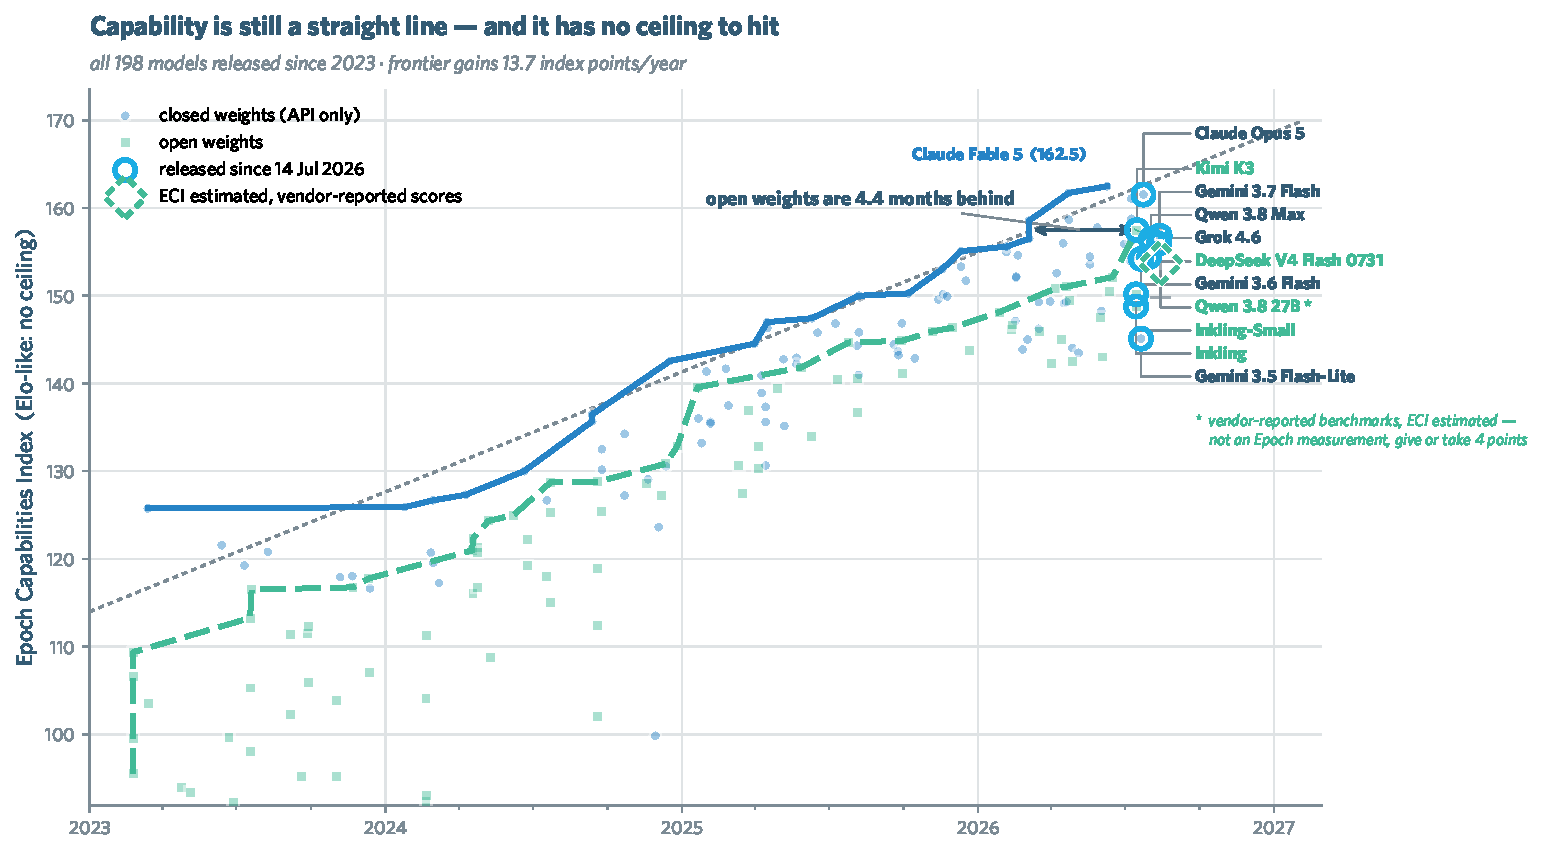
\includegraphics[height=0.50\textheight]{../model-progress/figures/fig3_eci_frontier.pdf}

  \vskip0.4em
  {\small{\color{tjo@darkteal}\bfseries 13 ECI points/year};
  {\small open weights ${\sim}6.9$ months behind (GLM-5.2)}}

  \vskip0.3em
  {\small\color{tjo@black!55} Epoch AI Benchmarking Hub, CC-BY, snapshot 2026-07-12}
\end{frame}

% --- Benchmark ladder / GPQA dead ---
\begin{frame}{Benchmarks saturate, then get replaced}
  \centering
  
\includegraphics[height=0.50\textheight]{../model-progress/figures/fig2_benchmark_ladder.pdf}

  \vskip0.4em
  {\small GPQA (PhD science QA) is {\color{tjo@darkteal}\bfseries dead at 94.6\%};
  research physics (CritPt) still at {\color{tjo@darkteal}\bfseries 32\%}}

  \vskip0.3em
  {\small\color{tjo@black!55} Epoch AI Benchmarking Hub, CC-BY, snapshot 2026-07-12}
\end{frame}

% --- Open-weight lag ---
\begin{frame}{You can run the frontier locally}
  \centering
  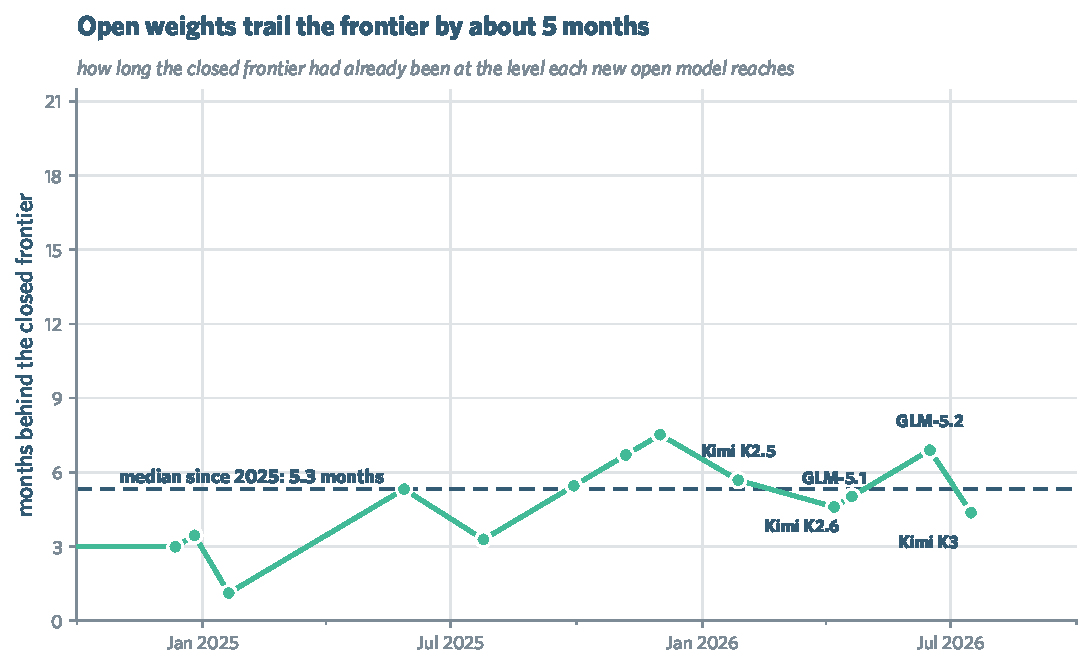
\includegraphics[height=0.50\textheight]{../model-progress/figures/fig5_open_weight_lag.pdf}

  \vskip0.4em
  {\small Run frontier-minus-7-months physics locally:
  {\color{tjo@darkteal}\bfseries no vendor lock-in}}

  \vskip0.3em
  {\small\color{tjo@black!55} Epoch AI Benchmarking Hub, CC-BY, snapshot 2026-07-12}
\end{frame}

% --- The renaissance expert (GC deck, working-tree version) ---
\begin{frame}{The renaissance expert}
  \vfill
  \centering
  \begin{tikzpicture}[every node/.style={align=center}]
    \node[tjo box, minimum width=4cm, minimum height=2cm, font=\small] (old) at (-4,0) {%
      {\bfseries\normalsize\color{tjo@darkteal} Old cost structure}\\[4pt]
      Years of apprenticeship\\[2pt]
      Deep, slow immersion\\[2pt]
      One domain per career
    };

    \node[tjo box fill, minimum width=4cm, minimum height=2cm, font=\small] (new) at (4,0) {%
      {\bfseries\normalsize\color{tjo@darkteal} New cost structure}\\[4pt]
      Hours to operational competence\\[2pt]
      Implementation $\approx$ free\\[2pt]
      Portfolio across domains
    };

    \draw[tjo arrow, line width=2pt]
      (old.east) -- (new.west)
      node[midway, above=10pt, font=\footnotesize, text=tjo@black!60] {agentic AI};
  \end{tikzpicture}

  \vskip1em
  {\normalsize\color{tjo@darkteal}\bfseries
    When execution is commoditized, the bottleneck shifts to problem formulation}
  \vfill
\end{frame}

% =====================================================================
% PART 7: THE HARDER PROBLEM
% =====================================================================

\sectiondivider{The harder problem}

% --- Why LLMs fail at research (GC deck) ---
\begin{frame}{Why LLMs fail at research}
  \vfill
  \centering
  \begin{tikzpicture}
    \node[tjo box fill, minimum width=4cm, minimum height=2cm, font=\small] (undergrad) at (-4,0) {%
      {\bfseries\normalsize\color{tjo@darkteal} Undergraduate}\\[4pt]
      Every step spelled out\\[2pt]
      Pedagogical structure\\[2pt]
      {\color{tjo@cyan} LLMs excel}
    };

    \node[tjo box, minimum width=4cm, minimum height=2cm, font=\small] (research) at (4,0) {%
      {\bfseries\normalsize\color{tjo@darkteal} Research}\\[4pt]
      ``By standard arguments''\\[2pt]
      Compressed communication\\[2pt]
      {\color{red!70!black} LLMs fail}
    };

    \draw[tjo arrow, line width=2pt]
      (undergrad.east) -- (research.west)
      node[midway, above=10pt, font=\footnotesize, text=tjo@black!60] {phase transition};
  \end{tikzpicture}

  \vskip1em
  {\normalsize\color{tjo@darkteal}\bfseries
    Models reproduce the texture of expertise, not the logic beneath it}
  \vfill
\end{frame}

% NEW (SPEC-EXTENSION B1)
\begin{frame}{Why structure a proof?}
  \vfill
  \centering
  {\fontsize{17}{23}\selectfont\itshape\color{tjo@black!70}
    ``By linearity \ldots\ and therefore \ldots\\[0.2em]
      which contradicts \ldots\ hence the result follows''}

  \vskip1.3em
  \begin{flushleft}
  \hspace{1.5em}Prose hides the gap

  \vskip0.6em
  \hspace{1.5em}When someone pushes back, \emph{which} step was wrong?

  \vskip0.6em
  \hspace{1.5em}Even a five-line argument can conceal it
  \end{flushleft}

  \vskip1.0em
  {\color{tjo@darkteal}\bfseries
    A proof you cannot point at is a proof you cannot check}
  \vfill
\end{frame}

% NEW (SPEC-EXTENSION B2)
\begin{frame}{Lamport structured proofs}
  \vfill
  \begin{flushleft}
  \hspace{1.5em}Every assertion gets a hierarchical number: 1, 1.1, 1.1.1

  \vskip0.35em
  \hspace{1.5em}Justified by citing earlier steps --- or by its children

  \vskip0.35em
  \hspace{1.5em}\textbf{ASSUME} opens a scope, \textbf{CASE} branches,
  \textbf{QED} closes

  \vskip0.35em
  \hspace{1.5em}A leaf with no justification is an
  {\color{red!70!black}exposed gap}
  \end{flushleft}

  \vskip0.6em
  \centering
  \begin{tikzpicture}[every node/.style={align=center}]
    \node[tjo box fill, minimum width=4.0cm, minimum height=1.25cm,
          font=\footnotesize] at (-4.35,0) {%
      {\bfseries\small\color{tjo@darkteal} Auditable}\\[2pt]
      ``I don't believe 1.3.2''};
    \node[tjo box fill, minimum width=4.0cm, minimum height=1.25cm,
          font=\footnotesize] at (0,0) {%
      {\bfseries\small\color{tjo@darkteal} Modular}\\[2pt]
      refine sub-steps alone};
    \node[tjo box fill, minimum width=4.0cm, minimum height=1.25cm,
          font=\footnotesize] at (4.35,0) {%
      {\bfseries\small\color{tjo@darkteal} Gap-visible}\\[2pt]
      nothing hides};
  \end{tikzpicture}

  \vskip0.55em
  {\color{tjo@darkteal}\bfseries
    That is the entire formalism --- no logic syntax to learn}
  \vfill
\end{frame}

% NEW (SPEC-EXTENSION B3)
% Ledger rendering of the paper's worked example
% (structured-proofs.tex 908--951).
\begin{frame}{No-cloning, structured}
  \vskip0.1em
  \centering
  {\footnotesize
  \begin{tabular}{@{}l@{\hskip 0.7em}p{8.2cm}@{\hskip 0.5em}l@{}}
    \color{tjo@darkteal}\bfseries 1 &
      There is no unitary $U$ with
      $U\ket{\psi}\ket{0} = \ket{\psi}\ket{\psi}$ for all $\ket{\psi}$ &
      \\[0.25em]
    \hspace{0.9em}\color{tjo@darkteal}\bfseries 1.1 &
      \textbf{ASSUME} such a cloning unitary $U$ exists &
      {\scriptsize\color{tjo@black!50}[hypothesis]} \\[0.25em]
    \hspace{0.9em}\color{tjo@darkteal}\bfseries 1.2 &
      $U\ket{0}\ket{0} = \ket{00}$ \; and \; $U\ket{1}\ket{0} = \ket{11}$ &
      {\scriptsize\color{tjo@black!50}[1.1]} \\[0.25em]
    \hspace{0.9em}\color{tjo@darkteal}\bfseries 1.3 &
      $U\ket{+}\ket{0}
        = \tfrac{1}{\sqrt{2}}\bigl(\ket{00} + \ket{11}\bigr)$ &
      {\scriptsize\color{tjo@black!50}[linearity, 1.2]} \\[0.25em]
    \hspace{0.9em}\color{tjo@darkteal}\bfseries 1.4 &
      $U\ket{+}\ket{0} = \ket{+}\ket{+}
        = \tfrac{1}{2}\bigl(\ket{00}+\ket{01}+\ket{10}+\ket{11}\bigr)$ &
      {\scriptsize\color{tjo@black!50}[1.1]} \\[0.25em]
    \hspace{0.9em}\color{tjo@darkteal}\bfseries 1.5 &
      Contradiction: Schmidt rank $2 \neq 1$ (entangled vs.\ product) &
      {\scriptsize\color{tjo@black!50}[1.3, 1.4]} \\[0.25em]
    \hspace{0.9em}\color{tjo@darkteal}\bfseries 1.6 &
      \textbf{QED} no such $U$ exists &
      {\scriptsize\color{tjo@black!50}[1.5]} \\
  \end{tabular}}

  \vskip0.45em
  {\small\color{tjo@darkteal}\bfseries
    Doubt step 1.5? Expand it: 1.5.1, 1.5.2 ---
    the proof refines exactly where the sceptic pushes}

  \vskip0.25em
  {\footnotesize\color{tjo@black!55}
    each step is the independently checkable block error correction demands}
\end{frame}

% --- Adversarial verification (GC deck) ---
\begin{frame}{Adversarial verification}
  \vfill
  \centering
  \begin{tikzpicture}[node distance=2cm, every node/.style={align=center}]
    \node[tjo box fill, minimum width=3cm] (prover) {%
      \textbf{Prover}\\{\small constructs}};
    \node[tjo box fill, right=2cm of prover, minimum width=3cm] (verifier) {%
      \textbf{Verifier}\\{\small attacks}};
    \node[tjo box, fill=tjo@darkteal, text=white,
          right=2cm of verifier, minimum width=3cm] (formal) {%
      \textbf{Formaliser}\\{\small Lean proof}};

    \draw[tjo arrow] (prover) -- (verifier);
    \draw[tjo arrow] (verifier) -- (formal);
    \draw[tjo arrow, dashed, color=tjo@cyan, bend right=30]
      (verifier.north) to node[above, font=\small, text=tjo@cyan] {reject} (prover.north);
  \end{tikzpicture}

  \vskip1.5em
  {\color{tjo@darkteal}\bfseries
    Natural language is an inadequate verification mechanism}

  \vskip0.5em
  {\small\color{tjo@black!60} Formal proof = compiler for mathematics}
  \vfill
\end{frame}

% --- Vibefeld 1: molecular pedantry (NEW) ---
\begin{frame}{Vibefeld: molecular pedantry}
  \vfill
  \centering
  \begin{tikzpicture}[every node/.style={align=center}]
    \node[tjo box, minimum width=2.8cm, minimum height=1.5cm, font=\small] (claim)
      at (-5.0,0) {\textbf{Claim 1}\\{\small the theorem}};
    \node[tjo box fill, minimum width=2.8cm, minimum height=1.5cm, font=\small] (steps)
      at (0,0) {\textbf{1.1, 1.2, \ldots}\\{\small atomic steps}};
    \node[tjo box, fill=tjo@darkteal, text=white, minimum width=2.8cm, minimum height=1.5cm, font=\small] (val)
      at (5.0,0) {\textbf{Validated}\\{\small survived attack}};
    \draw[tjo arrow] (claim) -- (steps)
      node[midway, above=5pt, font=\scriptsize, text=tjo@black!60] {decompose};
    \draw[tjo arrow] (steps) -- (val)
      node[midway, above=5pt, font=\scriptsize, text=tjo@black!60] {challenge};
  \end{tikzpicture}

  \vskip0.8em
  \begin{flushleft}
  \hspace{1.5em}A natural-language proof, decomposed into a ledger of tiny numbered claims

  \vskip0.6em
  \hspace{1.5em}Each claim must survive adversarial challenge \emph{on its own}
  \end{flushleft}

  \vskip0.8em
  \centering
  {\color{tjo@darkteal}\bfseries A hallucinated proof has nowhere to hide}

  \vskip0.4em
  {\small\color{tjo@black!55} github.com/tobiasosborne/vibefeld}
  \vfill
\end{frame}

% --- Vibefeld 2: how trust accumulates (NEW) ---
\begin{frame}{Vibefeld: how trust accumulates}
  \vfill
  \begin{flushleft}
  \hspace{1.5em}\textbf{Provers propose}, \textbf{verifiers attack}:\\
  \hspace{1.5em}a claim is accepted only when every challenge is resolved

  \vskip0.7em
  \hspace{1.5em}Every proposal, challenge, and resolution lands in an\\
  \hspace{1.5em}append-only ledger: a full audit trail

  \vskip0.7em
  \hspace{1.5em}Assumptions stay visible:\\
  \hspace{1.5em}an \emph{admitted} claim taints everything that depends on it
  \end{flushleft}

  \vskip0.8em
  \centering
  {\color{tjo@darkteal}\bfseries Provers convince. Verifiers attack. Truth emerges.}
  \vfill
\end{frame}

% NEW (SPEC-EXTENSION B4)
\begin{frame}{Break the correlations}
  \vfill
  \centering
  \begin{tikzpicture}[every node/.style={align=center}]
    \node[tjo box fill, minimum width=3.4cm, minimum height=1.5cm,
          font=\small] (p) at (-4.7,0) {%
      \textbf{Prover}\\{\small model A}};
    \node[tjo box, minimum width=3.8cm, minimum height=1.5cm,
          font=\small] (art) at (0,0) {%
      \textbf{1, 1.1, 1.2 \ldots}\\{\small the numbered artifact}};
    \node[tjo box, fill=tjo@darkteal, text=white, minimum width=3.4cm,
          minimum height=1.5cm, font=\small] (v) at (4.7,0) {%
      \textbf{Verifier}\\{\small model B, other lab}};

    \draw[tjo arrow] (p) -- (art);
    \draw[tjo arrow] (art) -- (v);
    \node[font=\scriptsize, text=red!70!black] at (0,-1.25)
      {never the prover's reasoning};
  \end{tikzpicture}

  \vskip0.7em
  \begin{flushleft}
  \hspace{1.5em}Different labs, different training data, different blind spots

  \vskip0.5em
  \hspace{1.5em}Agents invoke each other as shell commands: this automates
  \end{flushleft}

  \vskip0.6em
  {\color{tjo@darkteal}\bfseries
    A blind spot shared by every fresh session of one model\\
    is often glaring to another}
  \vfill
\end{frame}

% NEW (SPEC-EXTENSION B5)
\begin{frame}{Defense in depth}
  \vfill
  \centering
  \begin{tikzpicture}[every node/.style={align=center}]
    \draw[tjo arrow, line width=2pt] (-6.5,0) -- (6.6,0);
    \node[tjo box fill, minimum width=2.9cm, minimum height=1.3cm,
          font=\footnotesize] at (-5.0,0) {one-shot\\prose};
    \node[tjo box fill, minimum width=2.9cm, minimum height=1.3cm,
          font=\footnotesize] at (-1.68,0) {Lamport\\tree};
    \node[tjo box fill, minimum width=2.9cm, minimum height=1.3cm,
          font=\footnotesize] at (1.68,0) {lemma DAG\\$+$ contracts};
    \node[tjo box, fill=tjo@darkteal, text=white, minimum width=2.9cm,
          minimum height=1.3cm, font=\footnotesize] at (5.0,0)
      {machine-\\checked};
    \node[font=\scriptsize, text=tjo@black!60] at (0,-1.15)
      {cheap and weak \quad$\longrightarrow$\quad costly and strong};
  \end{tikzpicture}

  \vskip0.7em
  \begin{flushleft}
  \hspace{1.5em}Formalisation is a spectrum, not a single act

  \vskip0.5em
  \hspace{1.5em}No layer is trustworthy alone --- but they fail in
  \emph{different} places
  \end{flushleft}

  \vskip0.9em
  {\color{tjo@darkteal}\bfseries
    An agent produces every layer almost for free}

  \vskip0.35em
  {\small\color{tjo@black!55}
    Swiss cheese / defense in depth (Reason 2000)}
  \vfill
\end{frame}

% --- The single point of failure (GC deck, working-tree version) ---
\begin{frame}{The single point of failure}
  \vfill
  \begin{flushleft}
  \hspace{1.5em}Code has compilers. Proofs have proof assistants.

  \vskip0.8em
  \hspace{1.5em}\textbf{Planning documents have nothing.}

  \vskip0.8em
  \hspace{1.5em}You can verify that code implements a spec

  \vskip0.8em
  \hspace{1.5em}You cannot verify that the spec addresses the right problem
  \end{flushleft}

  \vskip1em
  \centering
  {\small\color{tjo@darkteal}\bfseries
    The scarce resource is structural taste:
    knowing which problems are load-bearing and which are decorative}
  \vfill
\end{frame}

% --- Trust arc 1: the proverb ---
\statementslide{``Trust arrives on foot\\[0.3em]
  and leaves on horseback''\\[1em]
  {\fontsize{16}{20}\selectfont\mdseries Dutch proverb}}

% --- Trust arc 2: mental model (from the seminar deck) ---
\statementslide{A good mental model of an LLM:\\[0.8em]
  a slightly unhinged,\\[0.3em]
  hypermotivated MSc student\\[1em]
  {\fontsize{16}{22}\selectfont\mdseries
    brilliant, tireless, and never to be taken on trust}}

% --- Trust arc 3: the investigative mindset ---
\begin{frame}{How trust is actually built}
  \vfill
  \begin{flushleft}
  \hspace{1em}Trust is not granted; it is \textbf{verified} into existence

  \vskip0.8em
  \hspace{1em}The foundation is \textbf{ground truth}:

  \vskip0.3em
  \hspace{2.5em}{\small primary sources, raw data, the actual output}

  \vskip0.8em
  \hspace{1em}The masters of this: \textbf{investigative journalists}

  \vskip0.3em
  \hspace{2.5em}{\small every claim traced to a source, checked independently}
  \end{flushleft}

  \vskip1em
  \centering
  {\small\color{tjo@darkteal}\bfseries
    Cultivate the investigative mindset}
  \vfill
\end{frame}

% --- Limitations (GC deck) ---
\begin{frame}[plain,c]
  \centering
  {\fontsize{20}{28}\selectfont\color{tjo@darkteal}
  Every layer we built today has failure modes

  \vskip1.5em
  Context rot, hallucination, tool misuse, prompt fragility

  \vskip1.5em
  The human in the loop is not optional
  }
\end{frame}

% --- Outsourcing (replaces the automation spectrum) ---
\statementslide{You can outsource \textbf{cognition}\\[0.5em]
  but you can't outsource \emph{understanding}}

% --- Summary (GC deck, line 3 adjusted for filesystem) ---
\begin{frame}{Summary}
  \vfill
  \centering
  {\fontsize{15}{22}\selectfont
    \begin{tabular}{@{}l}
      \color{tjo@darkteal}\bfseries LLMs are stateless functions{\mdseries{}:not magic, not minds} \\[1.2em]
      \color{tjo@darkteal}\bfseries Agents are loops{\mdseries{}:scaffolding provides the action} \\[1.2em]
      \color{tjo@darkteal}\bfseries The filesystem is ground truth{\mdseries{}:persistent, checkable memory} \\[1.2em]
      \color{tjo@darkteal}\bfseries The human provides taste{\mdseries{}:technique over hype} \\
    \end{tabular}
  }
  \vfill
\end{frame}

% --- Call to action (NEW final slide) ---
\begin{frame}{Try it this week}
  \vfill
  \centering
  \begin{tikzpicture}[every node/.style={align=center}]
    \node[tjo box fill, minimum width=3.6cm, minimum height=2cm, font=\small] (cc) at (-4.4,0) {%
      {\bfseries\normalsize\color{tjo@darkteal} Claude Code}\\[5pt]
      terminal agent\\[2pt]{\small\color{tjo@black!55} anthropic}};
    \node[tjo box fill, minimum width=3.6cm, minimum height=2cm, font=\small] (cx) at (0,0) {%
      {\bfseries\normalsize\color{tjo@darkteal} Codex}\\[5pt]
      terminal agent\\[2pt]{\small\color{tjo@black!55} openai}};
    \node[tjo box fill, minimum width=3.6cm, minimum height=2cm, font=\small] (pi) at (4.4,0) {%
      {\bfseries\normalsize\color{tjo@darkteal} Pi via OpenRouter}\\[5pt]
      open-weight option\\[2pt]{\small\color{tjo@black!55} no vendor lock-in}};
  \end{tikzpicture}

  \vskip1.4em
  {\fontsize{18}{24}\selectfont\color{tjo@darkteal}\bfseries
    Bring a real research problem, not a toy}
  \vfill
\end{frame}

% NEW (SPEC-EXTENSION C1)
\begin{frame}{An afternoon suffices}
  \vfill
  \begin{flushleft}
  {\normalsize
  \hspace{1em}{\color{tjo@cyan}$\bullet$}\; Open a coding agent in a
    directory you care about

  \vskip0.4em
  \hspace{1em}{\color{tjo@cyan}$\bullet$}\; Write a \code{CLAUDE.md}
    recording your standards

  \vskip0.4em
  \hspace{1em}{\color{tjo@cyan}$\bullet$}\; Keep a worklog, and a directory
    holding every paper you cite

  \vskip0.4em
  \hspace{1em}{\color{tjo@cyan}$\bullet$}\; Write the lemma you are fighting
    as a Lamport tree

  \vskip0.4em
  \hspace{1em}{\color{tjo@cyan}$\bullet$}\; Set one agent to prove, a second
    to attack --- only then read it

  \vskip0.4em
  \hspace{1em}{\color{tjo@cyan}$\bullet$}\; Formalise the one step you trust
    least
  }
  \end{flushleft}

  \vskip0.8em
  \centering
  {\color{tjo@darkteal}\bfseries
    The first three need no programming at all}
  \vfill
\end{frame}

% NEW (TIMELINE G4)
% The timeline, extended.  Geometry: design doc SS5.
\begin{frame}[plain]
\begin{designframe}[%
  yr/.style={anchor=north, font=\fontsize{4.6}{5.8}\selectfont},
  cnum/.style={anchor=north west, text=tjo@cyan,
               font=\fontsize{13.1}{15}\selectfont\bfseries},
  ccap/.style={anchor=north west, align=left, text width=45mm,
               text=tjo@ink, font=\fontsize{5.5}{7.2}\selectfont},
]
  \dftitle{The timeline, extended}
  \node[anchor=north west, text=tjo@muted,
        font=\fontsize{5.3}{6.6}\selectfont] at (40,104)
    {Left of today: measured. Right of today: extrapolation, clearly
     labelled.};

  % ---------- axis ----------
  \draw[tjo@lightgrey, line width=0.25mm] (60,286) -- (1240,286);
  \foreach \x in {90,260,430,600,770,940,1110}
    \draw[tjo@rule, line width=0.175mm] (\x,286) -- (\x,294);
  \foreach \x/\y in {90/2023, 260/2024, 430/2025, 600/2026}
    \node[yr, text=tjo@faint] at (\x,298) {\y};
  \foreach \x/\y in {770/2027, 940/2028, 1110/2029}
    \node[yr, text=tjo@future] at (\x,298) {\y};

  % ---------- measured segment ----------
  \draw[tjo@darkteal, line width=0.425mm] (90,270) -- (710,183);
  \fill[tjo@darkteal] (90,270) circle[radius=0.5625mm];
  \node[rotate=8, anchor=west, text=tjo@darkteal,
        font=\fontsize{5.3}{6.6}\selectfont\bfseries] at (146,200)
    {measured capability --- 179 frontier models since 2023};

  % ---------- today ----------
  \draw[tjo@cyan, line width=0.175mm, opacity=0.8,
        dash pattern=on 0.375mm off 0.5mm] (710,183) -- (710,286);
  \node[anchor=south east, text=tjo@darkteal,
        font=\fontsize{4.6}{5.8}\selectfont\bfseries] at (704,176) {today};

  % ---------- extrapolation ----------
  \draw[tjo@cyan, line width=0.375mm,
        dash pattern=on 1.125mm off 0.875mm] (710,183) -- (1180,117);
  \foreach \x/\y in {860/162, 1010/141, 1160/120} {
    \filldraw[fill=white, draw=tjo@cyan, line width=0.3mm]
      (\x,\y) circle[radius=0.875mm];
    \node[anchor=south, text=tjo@cyan,
          font=\fontsize{6.7}{8.4}\selectfont\bfseries] at (\x,\y-12) {?};
  }
  \fill[white] (710,183) circle[radius=1.0625mm];
  \fill[tjo@darkteal] (710,183) circle[radius=0.75mm];
  \node[anchor=north, text=tjo@cyan,
        font=\fontsize{5.7}{7.2}\selectfont\bfseries\itshape] at (928,198)
    {the slope has not bent yet};

  % ---------- six number chips ----------
  \foreach \l/\t in {40/336, 450/336, 860/336, 40/432, 450/432, 860/432}
    \fill[tjo@cyan] (\l,\t) rectangle (\l+4,\t+84);

  \node[cnum] at (56,338) {$+$13.0 / yr};
  \node[ccap] at (56,381)
    {Epoch Capabilities Index ---\\ still linear, no ceiling in sight};
  \node[cnum] at (466,338) {94.6\%};
  \node[ccap] at (466,381)
    {GPQA Diamond, saturated ---\\ the expert humans sit at 69.7\%};
  \node[cnum] at (876,338) {32.3\%};
  \node[ccap] at (876,381)
    {CritPt research physics ---\\ \textbf{your} frontier is still wide open};
  \node[cnum] at (56,434) {${\sim}1000\times$};
  \node[ccap] at (56,477)
    {Cheaper per attempt than 2023 ---\\ so run it a hundred ways and check};
  \node[cnum] at (466,434) {\$2{,}000};
  \node[ccap] at (466,477)
    {Price of a decade-open\\ conjecture, August 2026};
  \node[cnum] at (876,434) {2 s $\to$ 12 h};
  \node[ccap] at (876,477)
    {Autonomous task horizon ---\\ doubling every 4--7 months};

  % ---------- bridge, payload, sub-payload ----------
  \node[anchor=north, align=center, text=tjo@muted,
        font=\fontsize{6}{7.6}\selectfont] at (640,534)
    {Who did well in software: not the people who denied it, not the
     people who surrendered to it ---\\
     the people who learned to specify, to check, and to own the result.};
  \node[anchor=north, text=tjo@darkteal,
        font=\fontsize{11.7}{14}\selectfont\bfseries] at (640,590)
    {What would you attempt if the tedious 90\% were free?};
  \node[anchor=north, text=tjo@cyan,
        font=\fontsize{8.1}{10}\selectfont\bfseries] at (640,650)
    {Aim there.};
\end{designframe}
\end{frame}

% NEW (SPEC-EXTENSION C2)
\begin{frame}[plain,c]
  \centering
  {\fontsize{24}{31}\selectfont\bfseries\color{tjo@darkteal}
    The slop cannon is charged\\[0.2em]
    whether we like it or not\\[0.6em]
    {\fontsize{19}{25}\selectfont\mdseries
      The only question is how it is aimed}\par}

  \vskip1.3em
  {\fontsize{15}{21}\selectfont\color{tjo@black!75}
    Aimed with discipline --- error-corrected, ground-truthed,\\
    adversarially checked --- it is the cheapest instrument for\\
    rigorous exploration the sciences have ever been handed\par}

  \vskip1.3em
  \slopcaption
\end{frame}

% =====================================================================
% BACKUP: the economics objection ("nobody makes money on LLMs")
% Source: ~/Projects/llm-economics/REPORT.md (deep-research synthesis,
% July 2026; 122 sources, 24 claims adversarially verified)
% =====================================================================
\appendix

\sectiondivider{Additional slides: but don't they lose money?}

% --- Backup 1: triangulating inference cost ---
\begin{frame}{Triangulating the true cost of inference}
  \vfill
  \centering
  {\footnotesize\color{tjo@black!70} independent estimators, combined in log-space:\; energy physics (lower bound) $\cdot$ GPU rental\\[2pt]
   $\cdot$ market prices (upper bound) $\cdot$ DeepSeek's disclosure $\cdot$ Epoch AI models $\cdot$ leaked P\&Ls}

  \vskip0.8em
  {\footnotesize
  \begin{tabular}{@{}lcc@{}}
    \toprule
    Model class & Cost per M output tokens & 68\% interval \\
    \midrule
    DeepSeek-V3 class (37B active, MLA) & \$0.35 & \$0.27--0.46 \\
    Frontier workhorse (GPT-5 / Sonnet class) & \$2.1 & \$1.2--3.7 \\
    Frontier flagship (Opus class) & \$8.5 & \$3.5--21 \\
    \bottomrule
  \end{tabular}}

  \vskip0.8em
  {\small\color{tjo@darkteal}\bfseries A typical chat query costs the provider $\sim$0.1 cents}

  \vskip2pt
  {\footnotesize\color{tjo@black!55} folklore: off $\sim$10x on energy (0.3\,Wh vs.\ ``3\,Wh''), $\sim$100x on cost}
  \vfill
\end{frame}

% --- Backup 2: margins ---
\begin{frame}{Prices vs.\ costs: the margins are real}
  \vfill
  \centering
  {\footnotesize
  \begin{tabular}{@{}lccc@{}}
    \toprule
    API product & Output price & Gross margin & $\Prob(>0)$ \\
    \midrule
    Claude Sonnet class & \$15\,/\,M & 86\% \; [57--95\%] & $>$99.9\% \\
    GPT-5 class & \$10\,/\,M & 79\% \; [35--93\%] & 99.7\% \\
    DeepSeek R1 (self-disclosed ``545\%'') & \$2.19\,/\,M & 84\% \; [73--90\%] & $\sim$100\% \\
    \bottomrule
  \end{tabular}}

  \vskip1.2em
  {\footnotesize\color{tjo@black!70} leaked P\&Ls agree:\; Anthropic $-94\%$ (2024) $\to$ mid-60s\% (Q1 2026), first profit Q2 2026;\\[2pt]
   OpenAI 28\% $\to$ 43\% while free users consume $\sim$half the inference bill}

  \vskip1.2em
  {\small\color{tjo@darkteal}\bfseries ``We're profitable on inference.'' --- Altman \qquad ``$>$50\%'' --- Amodei}
  \vfill
\end{frame}

% --- Backup 3: the honest fine print ---
\begin{frame}{The honest fine print}
  \vfill
  \centering
  {\small\color{tjo@darkteal}\bfseries Subscriptions}\\[2pt]
  {\footnotesize median \$20 subscriber costs \emph{cents}/month; power tiers bimodal --- rate limits cap the tail}

  \vskip0.6em
  {\small\color{tjo@darkteal}\bfseries What survives on the skeptic side}\\[2pt]
  {\footnotesize long-context cost floors $\cdot$ reasoning models burn 10--50x tokens/query $\cdot$ GPU rents \emph{rose} in 2026}

  \vskip0.6em
  {\small\color{tjo@darkteal}\bfseries The losses are real, but discretionary}\\[2pt]
  {\footnotesize OpenAI 2025 op.\ loss $\sim$\$21B $=$ R\&D \$19B $+$ training $\sim$\$8B, on \emph{positive} serving margins}

  \vskip0.7em
  {\small\color{tjo@darkteal}\bfseries Not failing to make money --- choosing to reinvest more than they earn}
  \vfill
\end{frame}


\end{document}
